%%%%%%%%%%%%%%%%%%%%%%%%%%%%%%%%%%%%%%%%%%%%%%%%%%%%%%%%%%%%%%%
\begin{frame}[t]
\frametitle{線形システム論詳解}
%-------------------------------------------------------------


前章では線形システム論（状態方程式で表されたシステムに対する極配置による状態フィードバック，２次形式評価関数を最小にする最適制御，オブザーバを用いた出力フィードバックの設計理論）に基づいて制御系を設計するために最低限必要な概念について概観した．
\\[3mm]

本章ではこれらについての数学的証明や，詳細な性質などについて説明する．これらは制御理論を研究（発展）させるものとして，最低限必要な知識となる．

\end{frame}

%%%%%%%%%%%%%%%%%%%%%%%%%%%%%%%%%%%%%%%%%%%%%%%%%%%%%%%%%%%%%%%
\begin{frame}[t]
\frametitle{2.1 極配置問題と可制御正準形}
%-------------------------------------------------------------


\section{極配置問題と可制御正準形 \label{sec_c_canonical}}
%---------------------------------------------------------------------------
１入力可制御なシステムの極配置はシステムが可制御正準形であれば容易であることを1.9.1節で示した．
\\[3mm]

ここでは可制御な状態方程式を可制御正準形に変換する座標変換の求め方について述べる．
\\[3mm]

また，可制御正準形で設計されたフィードバックを元の状態のフィードバックにどのように変換するかについても述べる．
\end{frame}

%%%%%%%%%%%%%%%%%%%%%%%%%%%%%%%%%%%%%%%%%%%%%%%%%%%%%%%%%%%%%%%
\begin{frame}[t]
\frametitle{2.1.1 1入力可制御正準形への変換}
%-------------------------------------------------------------

\subsection{1入力可制御正準形への変換}

可制御な１入力状態方程式
\begin{align}
 \frac{dx}{dt} &= Ax + Bu
\nonumber
\end{align}
を考える．この状態方程式を可制御正準形に変換する座標変換は次で与えられる．システムは1入力で可制御を仮定しているから
\begin{equation}
 V = \left(\begin{array}{cccccc}
            B & A B & A^2 B & \cdots & A^{n-2} B & A^{n-1} B
	   \end{array}\right)
\end{equation}
は正則になる．いまこの逆行列の行ベクトルを
\begin{equation}
 V^{-1} = \left(\begin{array}{c}
	     l_1^T \\
		 l_2^T \\
		 l_3^T \\
		 \vdots \\
		 l_{n-1}^T \\
		 l_n^T
		\end{array}\right)
\end{equation}
と表わすことにする．


\end{frame}

%%%%%%%%%%%%%%%%%%%%%%%%%%%%%%%%%%%%%%%%%%%%%%%%%%%%%%%%%%%%%%%
\begin{frame}[t]
\frametitle{2.1.1 1入力可制御正準形への変換}
%-------------------------------------------------------------

このうちの$l_n^T$を用いて座標変換行列$T$を
\begin{align}
 T &= W^{-1} \\
 W &= \left(\begin{array}{c}
	      l_n^T     \\
	      l_n^T A   \\
	      l_n^T A^2 \\
	      \vdots    \\
	      l_n^T A^{n-2} \\
	      l_n^T A^{n-1}
	     \end{array}\right)
\end{align}
とすればシステムは可制御正準形に変換される．
\end{frame}

%%%%%%%%%%%%%%%%%%%%%%%%%%%%%%%%%%%%%%%%%%%%%%%%%%%%%%%%%%%%%%%
\begin{frame}[t]
\frametitle{2.1.1 1入力可制御正準形への変換(証明)}
%-------------------------------------------------------------


\noindent
(証明)

逆行列の定義より
\begin{align}
 V^{-1} V = I
\end{align}
が成り立つ．これを要素で表せば
\begin{align}
	&
	\left(\begin{array}{c}
		 l_1^T \\
		 l_2^T \\
		 l_3^T \\
		 \vdots \\
		 l_{n-1}^T \\
		 l_n^T
	\end{array}\right)
	\left(\begin{array}{cccccc}
            B & A B & A^2 B & \cdots &A^{n-2}B &  A^{n-1} B
	\end{array}\right)
\nonumber\\
	& \hspace*{1cm}=
	\left(\begin{array}{cccccc}
		 *       & *         & *           & \cdots & *              & *              \\
		 *       & *         & *           & \cdots & *              & *              \\
		 *       & *         & *           & \cdots & *              & *              \\
		 \vdots  & \vdots    & \vdots      &        & \vdots         & \vdots         \\
		 *       & *         & *           & \cdots & *              & *              \\
		 l_n^T B & l_n^T A B & l_n^T A^2 B & \cdots & l_n^T A^{n-2}B & l_n^T A^{n-1}B
	\end{array}\right)
\nonumber\\
	& \hspace*{1cm}=
	\left(\begin{array}{cccccc}
		 *       & *         & *           & \cdots & *              & *              \\
		 *       & *         & *           & \cdots & *              & *              \\
		 *       & *         & *           & \cdots & *              & *              \\
		 \vdots  & \vdots    & \vdots      &        & \vdots         & \vdots         \\
		 *       & *         & *           & \cdots & *              & *              \\
		 0       & 0         & 0           & \cdots & 0              & 1
	\end{array}\right)
\end{align}
\end{frame}

%%%%%%%%%%%%%%%%%%%%%%%%%%%%%%%%%%%%%%%%%%%%%%%%%%%%%%%%%%%%%%%
\begin{frame}[t]
\frametitle{2.1.1 1入力可制御正準形への変換(証明)}
%-------------------------------------------------------------

であるから
\begin{align}
		 l_n^T B =0 
		 ,\ \ 
		 l_n^T A B =0
		 ,\ \ 
		 l_n^T A^2 B =0
		 ,\ \ 
		 \cdots 
		 ,\ \ 
		 l_n^T A^{n-2}B =0
		 ,\ \ 
		 l_n^T A^{n-1}B =1
\label{eq:controller_canonica_form_proof1}
\end{align}
となる．いま，スカラー関数として
\begin{align}
	\phi(x) = l_n^T x
\end{align}
を定義する．
\end{frame}

%%%%%%%%%%%%%%%%%%%%%%%%%%%%%%%%%%%%%%%%%%%%%%%%%%%%%%%%%%%%%%%
\begin{frame}[t]
\frametitle{2.1.1 1入力可制御正準形への変換(証明)}
%-------------------------------------------------------------
$\phi$の時間微分を繰り返せば(\ref{eq:controller_canonica_form_proof1})を用いて
\begin{align}
	\phi &= l_n^T x
\nonumber\\
	\frac{d \phi}{dt} 
	& = \frac{d}{dt} l_n^T x 
	= l_n^T \frac{dx}{dt} 
	= l_n^T (Ax+Bu) 
	= l_n^T A x + l_n^T Bu 
	= l_n^T A x 
\nonumber\\
	\frac{d^2 \phi}{dt^2} 
	& = \frac{d}{dt} \ \frac{d \phi}{dt}
	= \frac{d}{dt} l_n^T A x 
\nonumber \\ &
	= l_n^T A \frac{dx}{dt} 
	= l_n^T A (Ax+Bu) 
	= l_n^T A^2 x + l_n^T A Bu 
	= l_n^T A^2 x 
\nonumber\\
	\vdots
\\
	\frac{d^{n-1} \phi}{dt^{n-1}} 
	& = l_n^T A^{n-2} \frac{dx}{dt} 
	= l_n^T A^{n-2} (Ax+Bu) 
	= l_n^T A^{n-1} x + l_n^T A^{n-2} Bu 
	= l_n^T A^{n-1} x 
\nonumber\\
	\frac{d^{n} \phi}{dt^{n}} 
	& = l_n^T A^{n-1} \frac{dx}{dt} 
	= l_n^T A^{n-1} (Ax+Bu) 
	= l_n^T A^{n} x + l_n^T A^{n-1} Bu 
	= l_n^T A^{n} x + u
\nonumber
\end{align}
を得る．
\end{frame}

%%%%%%%%%%%%%%%%%%%%%%%%%%%%%%%%%%%%%%%%%%%%%%%%%%%%%%%%%%%%%%%
\begin{frame}[t]
\frametitle{2.1.1 1入力可制御正準形への変換(証明)}
%-------------------------------------------------------------
これは$\phi$を$n$階微分して初めて$u$の影響が出てきたことを示している．いま，新しい状態$\bar{x}$として
\begin{align} 
	\bar{x}
	& =
	\left(\begin{array}{c}
	     \bar{x}_1 \\
	     \bar{x}_2 \\
	     \bar{x}_3 \\
		 \vdots \\
	     \bar{x}_{n-1} \\
	     \bar{x}_n
	\end{array}\right)
	=
	\left(\begin{array}{c}
	     \phi \\
	     d \phi /dt \\
	     d^2 \phi /dt^2 \\
		 \vdots \\
	     d^{n-2} \phi /dt^{n-2} \\
	     d^{n-1} \phi /dt^{n-1}
	\end{array}\right)
	=
	\left(\begin{array}{c}
	     l_n^T x \\
	     l_n^T A x \\
	     l_n^T A^2 x \\
		 \vdots \\
	     l_n^T A^{n-2} x \\
	     l_n^T A^{n-1} x
	\end{array}\right)
	=
	\left(\begin{array}{c}
	     l_n^T  \\
	     l_n^T A  \\
	     l_n^T A^2  \\
		 \vdots \\
	     l_n^T A^{n-2}  \\
	     l_n^T A^{n-1} 
	\end{array}\right)
	x
\nonumber \\ &
	= Wx
	= T^{-1}x
\end{align}
と定義する($x = T \bar{x}$)．
\end{frame}

%%%%%%%%%%%%%%%%%%%%%%%%%%%%%%%%%%%%%%%%%%%%%%%%%%%%%%%%%%%%%%%
\begin{frame}[t]
\frametitle{2.1.1 1入力可制御正準形への変換(証明)}
%-------------------------------------------------------------
座標変換の定義と(\ref{eq:controller_canonica_form_proof1})より以下の時間微分は明らかである．
\begin{align}
	\frac{d \bar{x}}{dt}
	& =
	\left(\begin{array}{c}
	     d \phi /dt \\
	     d^2 \phi /dt^2 \\
	     d^3 \phi /dt^3 \\
		 \vdots \\
	     d^{n-1} \phi /dt^{n-1} \\
	     d^{n} \phi /dt^{n}
	\end{array}\right)
	=
	\left(\begin{array}{c}
	     \bar{x}_2 \\
	     \bar{x}_3 \\
	     \bar{x}_4 \\
		 \vdots \\
	     \bar{x}_{n} \\
	     l_n^T A^{n} x + u
	\end{array}\right)
	=
	\left(\begin{array}{c}
	     \bar{x}_2 \\
	     \bar{x}_3 \\
	     \bar{x}_4 \\
		 \vdots \\
	     \bar{x}_{n} \\
	     l_n^T A^{n} T \bar{x} + u
	\end{array}\right)
\end{align}
これを行列で表せば
\begin{align}
 \frac{d}{dt}
  \left(\begin{array}{c}
     \bar{x}_1 \\
	 \bar{x}_2 \\
	 \bar{x}_3 \\
	 \vdots \\
	 \bar{x}_{n-1} \\
	 \bar{x}_n
	\end{array}\right)
  &=
  \left(\begin{array}{cccccc}
     0      & 1      & 0      & 0      & \cdots & 0     \\
     0      & 0      & 1      & 0      & \ddots & 0     \\
	 0      & 0      & 0      & \ddots & \ddots & \vdots\\
	 \vdots & \vdots & \vdots & \ddots & 1      & 0     \\
	 0      & 0      & 0      & \cdots & 0      & 1     \\
	 *      & *      & *      & \cdots & *      & *
	\end{array}\right)
  \left(\begin{array}{c}
     \bar{x}_1 \\
	 \bar{x}_2 \\
	 \bar{x}_3 \\
	 \vdots \\
	 \bar{x}_{n-1} \\
	 \bar{x}_n
	\end{array}\right)
  +
  \left(\begin{array}{c}
     0 \\
	 0 \\
	 0 \\
	 \vdots \\
	 0 \\
	 1
	\end{array}\right)
  u 
\end{align}
と可制御正準形で表される．

\end{frame}

%%%%%%%%%%%%%%%%%%%%%%%%%%%%%%%%%%%%%%%%%%%%%%%%%%%%%%%%%%%%%%%
\begin{frame}[t]
\frametitle{2.1.1 1入力可制御正準形への変換(演習)}
%-------------------------------------------------------------

\noindent
{\bf[演習]}\nopagebreak

次のシステムを可制御正準形に変換せよ．
\begin{align}
 \frac{d}{dt}
  \left(\begin{array}{c}
     {x}_1 \\
	 {x}_2 \\
	 {x}_3 
	\end{array}\right)
  &=
  \left(\begin{array}{ccc}
     0      & 2      & 3     \\
     1      & -1     & -1    \\
	 0      & 1      & 1     
	\end{array}\right)
  \left(\begin{array}{c}
     {x}_1 \\
	 {x}_2 \\
	 {x}_3 
	\end{array}\right)
  +
  \left(\begin{array}{c}
     1 \\
	 0 \\
	 0 
	\end{array}\right)
  u 
\nonumber \\
	y &= 
  \left(\begin{array}{ccc}
     0      & 1      & 1 
	\end{array}\right)
  \left(\begin{array}{c}
     {x}_1 \\
	 {x}_2 \\
	 {x}_3 
	\end{array}\right)
\nonumber 
\end{align}
\end{frame}

%%%%%%%%%%%%%%%%%%%%%%%%%%%%%%%%%%%%%%%%%%%%%%%%%%%%%%%%%%%%%%%
\begin{frame}[t]
\frametitle{2.1.2 座標変換とフィードバック}
%-------------------------------------------------------------


\subsection{座標変換とフィードバック}

状態方程式
\begin{align}
 \frac{dx}{dt} &= Ax + Bu
\nonumber
\end{align}
を座標変換
\begin{align}
 x = T\bar{x}
\end{align}
により可制御正準形に変換し，
\begin{align}
 \frac{ d \bar{x}}{dt} = T^{-1} A T \bar{x} + T^{-1} B u = \bar{A} \bar{x} + \bar{B} u
\end{align}
1.9.1節で述べた可制御正準形に対する極配置手法を用いることにより状態フィードバックを
\begin{align}
 u =\bar{F} \bar{x} + v
\end{align}
と設計したとしよう．
\end{frame}

%%%%%%%%%%%%%%%%%%%%%%%%%%%%%%%%%%%%%%%%%%%%%%%%%%%%%%%%%%%%%%%
\begin{frame}[t]
\frametitle{2.1.2 座標変換とフィードバック}
%-------------------------------------------------------------
この状態$\bar{x}$のフィードバックは元の状態$x$の状態フィードバックとしては$\bar{x} = T^{-1} x$を用いて
\begin{align}
 u = \bar{F} \bar{x} + v = \bar{F} T^{-1} x + v = F x + v, \ \ \ F=\bar{F} T^{-1}, \ \bar{F} = FT
\end{align}
と表される．実際に$\bar{x}$と$x$でのフィードバック系の特性多項式を計算すれば
\begin{align}
  \det (s I - \bar{A} - \bar{B} \bar{F}) 
  &=
  \det \{(s I - T^{-1} A T - T^{-1} B F T) \} 
\nonumber \\
  &=
  \det \{T^{-1}(s I -  A -  B F ) T\} 
\nonumber \\
  &=
  \det (T^{-1}) \det (s I - A - B F) \det (T) 
\nonumber \\
  &=
  \det (s I - A - B F) 
\end{align}
となり，この$F$が元の状態方程式に対して極配置を満たしていることが分かる．
\end{frame}

%%%%%%%%%%%%%%%%%%%%%%%%%%%%%%%%%%%%%%%%%%%%%%%%%%%%%%%%%%%%%%%
\begin{frame}[t]
\frametitle{2.1.2 座標変換とフィードバック}
%-------------------------------------------------------------

Fig,\ref{fig:poleplace}は座標変換によりシステムを可制御正準形に変換してから可制御正準形に対する極配置手法を用いる設計法の概要を示している．
\begin{figure}
\begin{center}
\scalebox{0.8}{
\input{../figure/summary.pstex_t}
}
  \caption{極配置問題の解法}
  \label{fig:poleplace}
\end{center}
\end{figure}

\end{frame}

%%%%%%%%%%%%%%%%%%%%%%%%%%%%%%%%%%%%%%%%%%%%%%%%%%%%%%%%%%%%%%%
\begin{frame}[t]
\frametitle{2.2 １入力システムの正準形}
%-------------------------------------------------------------

%---------------------------------------------------------------------------
\section{１入力システムの正準形}
%---------------------------------------------------------------------------

1.9.1節の極配置問題で述べたように可制御正準形は状態フィードバックを見通しよく設計できる状態方程式であることがわかる．実はこのような正準形と呼ばれるものは可制御正準形以外にも存在する．
\\[3mm]

1.4節では１入力１出力伝達関数を可制御正準形で表したが，ここでは別の正準形で表すことを考える．
\\[3mm]

1.4節と同様に一入出力の伝達関数
\begin{equation}
 G(s) =
  \frac{b_{n-1} s^{n-1} + b_{n-2} s^{n-2} + \cdots + b_1 s + b_0}
  {s^n + a_{n-1} s^{n-1} + a_{n-2} s^{n-2} + \cdots + a_1 s + a_0}
  + d
\end{equation}
を考える．このシステムの状態空間表現は一意ではない（座標変換分の自由度がある）．しかし，その中でも次の3つは有用である．

\end{frame}

%%%%%%%%%%%%%%%%%%%%%%%%%%%%%%%%%%%%%%%%%%%%%%%%%%%%%%%%%%%%%%%
\begin{frame}[t]
\frametitle{2.2.1可制御正準形}
%-------------------------------------------------------------
\subsection{可制御正準形}
%---------------------------------------------------------------------------

1.4節参照．状態方程式で表されたシステムを可制御正準形に変換する座標変換は2.1節参照．

\end{frame}

%%%%%%%%%%%%%%%%%%%%%%%%%%%%%%%%%%%%%%%%%%%%%%%%%%%%%%%%%%%%%%%
\begin{frame}[t]
\frametitle{2.2.2 可観測正準形}
%-------------------------------------------------------------
\subsection{可観測正準形}
%---------------------------------------------------------------------------

1入出力伝達関数は明らかにスカラー関数であるから次が成り立つ．
\begin{align}
 G(s)^T = G(s)
\end{align}
つまり$G(s)$が状態方程式$(A,B,C,D)$で与えられているとき
\begin{align}
 G(s) &= G(s)^T = \{ C(sI-A)^{-1}B + D\} ^T = \{ B^T (sI-A)^{-T} C^T + D^T\} 
\nonumber\\
 &= B^T \{(sI-A)^{T}\}^{-1} C^T + D^T = B^T (sI - A^{T})^{-1} C^T + D^T
\end{align}
となる．(ここで$M^{-T} = (M^{T})^{-1} = (M^{-1})^T$を用いた)．

\end{frame}

%%%%%%%%%%%%%%%%%%%%%%%%%%%%%%%%%%%%%%%%%%%%%%%%%%%%%%%%%%%%%%%
\begin{frame}[t]
\frametitle{2.2.2 可観測正準形}
%-------------------------------------------------------------


いま，$(A,B,C,D)$として可制御正準形を用いれば伝達関数が次の状態方程式で表されることがわかる．
\begin{align}
 \frac{d}{dt}
  \left(\begin{array}{c}
         x_1 \\
	 x_2 \\
	 \vdots \\
	 x_{n-1} \\
	 x_n
	\end{array}\right)
  &=
  \left(\begin{array}{ccccc}
     0      & 0      & \cdots & 0      & -a_0  \\
	 1      & 0      & \cdots & 0      & -a_1 \\
     0      & 1      & \ddots & \vdots & \vdots \\
	 \vdots & \ddots & \ddots & 0      & -a_{n-2} \\
	 0      & \cdots & 0      & 1      & -a_{n-1}
	\end{array}\right)
  \left(\begin{array}{c}
	 x_1 \\
	 x_2 \\
	 \vdots \\
	 x_{n-1} \\
	 x_n
	\end{array}\right)
  +
  \left(\begin{array}{c}
     b_0 \\
	 b_1 \\
	 \vdots \\
	 b_{n-2} \\
	 b_{n-1}
	\end{array}\right)
  u \label{eq:canoform_o}\\
y &=
 \left(\begin{array}{ccccc}
        0 & 0 & \cdots & 0 & 1
       \end{array}\right)
 \left(\begin{array}{c}
        x_1 \\
	x_2 \\
	\vdots \\
	x_{n-1} \\
	x_n
       \end{array}\right)
 + d u
\end{align}
これを{\bf {可観測正準形}(observer canonical form)}と呼ぶ．
\end{frame}

%%%%%%%%%%%%%%%%%%%%%%%%%%%%%%%%%%%%%%%%%%%%%%%%%%%%%%%%%%%%%%%
\begin{frame}[t]
\frametitle{2.2.2 可観測正準形}
%-------------------------------------------------------------

１入出力可観測な状態方程式を可観測正準形に変換する座標変換は
\begin{enumerate}
  \item 状態方程式の双対システムを求める．
  \item 双対システムを可制御正準形に変換する．
  \item 可制御正準形の双対システムが可観測正準形となる．
  \item 双対システムの座標変換行列$T$の逆転置$T^{-T}$が元の状態方程式を直接，可観測正準形に変換する座標変換となる．
\end{enumerate}
により求めることができる．このシステムを用いればオブザーバの極配置問題が（状態フィードバックの極配置問題を可制御正準形を用いて解くように）容易に解ける．


\end{frame}

%%%%%%%%%%%%%%%%%%%%%%%%%%%%%%%%%%%%%%%%%%%%%%%%%%%%%%%%%%%%%%%
\begin{frame}[t]
\frametitle{2.2.3 対角正準形}
%-------------------------------------------------------------
\subsection{対角正準形}
%---------------------------------------------------------------------------

極が重複しないと仮定して伝達関数$G(s)$を部分分数展開して次で表す．
\begin{align}
 G(s) = \frac{\beta_1}{s-\lambda_1} + \frac{\beta_2}{s-\lambda_2} + \cdots 
        \frac{\beta_n}{s-\lambda_n} + d
\end{align}
これを状態方程式に表すと次の{\bf {対角正準形}(diagonal canonical form)}に表される．
\begin{align}
 \frac{d}{dt}
  \left(\begin{array}{c}
         x_1 \\
	 x_2 \\
	 \vdots \\
	 x_n
	\end{array}\right)
  &=
  \left(\begin{array}{cccc}
     \lambda_1 & 0         & \cdots & 0  \\
	 0         & \lambda_2 & \ddots & \vdots \\
	 \vdots    & \ddots    & \ddots & 0 \\
	 0         & \cdots    & 0      & \lambda_n
	\end{array}\right)
  \left(\begin{array}{c}
	 x_1 \\
	 x_2 \\
	 \vdots \\
	 x_n
	\end{array}\right)
  +
  \left(\begin{array}{c}
     1 \\
	 1 \\
	 \vdots \\
	 1
	\end{array}\right)
  u \label{eq:canoform_d}\\
y &=
 \left(\begin{array}{cccc}
        \beta_1 & \beta_2 & \cdots & \beta_{n}
       \end{array}\right)
 \left(\begin{array}{c}
        x_1 \\
	x_2 \\
	\vdots \\
	x_n
       \end{array}\right)
 + d u
\end{align}
\end{frame}

%%%%%%%%%%%%%%%%%%%%%%%%%%%%%%%%%%%%%%%%%%%%%%%%%%%%%%%%%%%%%%%
\begin{frame}[t]
\frametitle{2.2.3 対角正準形}
%-------------------------------------------------------------

例えば，近似微分要素を表す伝達関数は
\begin{align}
 \frac{Ts}{Ts+1} = \frac{s}{s+\frac{1}{T}}
 = \frac{-\frac{1}{T}}{s+\frac{1}{T}} + 1
\end{align}
となるので，状態方程式で表すと
\begin{align}
 \frac{dx}{dt} &= -\frac{1}{T} x + 1u \\
 y             &= -\frac{1}{T} x + 1u
\end{align}
となる．

\end{frame}

%%%%%%%%%%%%%%%%%%%%%%%%%%%%%%%%%%%%%%%%%%%%%%%%%%%%%%%%%%%%%%%
\begin{frame}[t]
\frametitle{2.3 最適制御：証明と性質}
%-------------------------------------------------------------

\section{最適制御：証明と性質}
%---------------------------------------------------------------------------

ここでは1.9.3節で扱った最適制御の数学的証明と，最適制御について知っておくべき性質について述べる．
\\[3mm]

まず，最適制御の安定性を証明するために必要なリアプノフ関数について述べるが，その前に正定行列について復習しておこう．

\end{frame}

%%%%%%%%%%%%%%%%%%%%%%%%%%%%%%%%%%%%%%%%%%%%%%%%%%%%%%%%%%%%%%%
\begin{frame}[t]
\frametitle{（行列論：復習）対称行列，正定行列，半正定行列}
%-------------------------------------------------------------

\subsubsection{（行列論：復習）対称行列，正定行列，半正定行列}
\noindent
{\bf \underline{正定行列}}

正方な実行列$A$は$A^T=A$を満たすとき{\bf \underline{対称行列(symmetric matrix)}}であるという．対称行列は$T^T T=I$を満たす{\bf \underline{直交行列(orthogonal matrix)}} $T$で対角化される($T^T A T = \Lambda$:対角行列).
\\[3mm]

実行列$P$が{\bf \underline{正定行列(positive definite matrix)}}であるとは$P$が対称かつ以下を満たすことである．
\begin{eqnarray}
	x^T P x > 0, \ \ \ x \neq 0
\end{eqnarray}
$P$が正定行列であるとき以下のようにあらわす．
\begin{eqnarray}
	P>0
\end{eqnarray}
正定行列の例($ P = I $)
\begin{eqnarray}
	x^T I x = x^T x = \vert x \vert^2 > 0, \ \ \ x \neq 0
\end{eqnarray}
\end{frame}

%%%%%%%%%%%%%%%%%%%%%%%%%%%%%%%%%%%%%%%%%%%%%%%%%%%%%%%%%%%%%%%
\begin{frame}[t]
\frametitle{（行列論：復習）対称行列，正定行列，半正定行列}
%-------------------------------------------------------------

\noindent
{\bf \underline{正定行列の性質}}
\begin{itemize}
  \item $P$が正定$\Leftrightarrow$ $P$の{\underline{固有値はすべて正}}
  \item $P$が正定$\Leftrightarrow$ $\exists M$：正則行列 s.t. {\bf \underline{$P = M^T M$}}　（$M$を$P^{\frac{1}{2}}$とあらわすことがある）\\
  	$P=M^TM$の場合，$x^T P x = x^T M^T M x = (Mx)^T Mx $．
  	$Mx=y$と定義すれば$x^T P x = y^T y = \vert y \vert^2>0$．\\
  	$(y \neq 0 \ \ \Leftrightarrow \ \ x \neq 0)$
  \item $P$が正定$\Leftrightarrow$ $P$の主座小行列式がすべて正（{\bf \underline{シルベスターの判別条件}}）
  \item $P$が正定$\Leftrightarrow$ {\underline{$P^{-1}$も正定}}
\end{itemize}
\end{frame}


%%%%%%%%%%%%%%%%%%%%%%%%%%%%%%%%%%%%%%%%%%%%%%%%%%%%%%%%%%%%%%%
\begin{frame}[t]
\frametitle{（行列論：復習）対称行列，正定行列，半正定行列}
%-------------------------------------------------------------

\noindent
{\bf \underline{半正定行列}}

実行列$P$が{\bf \underline{半正定行列(positive semi-definite matrix)}}であるとは$P$が対称かつ以下を満たすことである．
\begin{eqnarray}
	x^T P x \geq 0
\end{eqnarray}
半正定行列は準正定行列または{\bf \underline{非負定行列(non-negative definite matrix)}}と呼ばれることもある．$P$が半正定行列であるとき以下のようにあらわす．
\begin{eqnarray}
	P \geq 0
\end{eqnarray}
半正定行列の例($ P = \left(\begin{array}{cc} 1 & 0 \\ 0 & 0 \end{array}\right) $)
\begin{eqnarray}
	x^T P x = 
	\left(\begin{array}{cc} x_1 & x_2 \end{array}\right)
	\left(\begin{array}{cc} 1 & 0 \\ 0 & 0 \end{array}\right)
	\left(\begin{array}{c}  x_1 \\ x_2 \end{array}\right)
	=
	x_1^2 \geq 0
\end{eqnarray}
\end{frame}



%%%%%%%%%%%%%%%%%%%%%%%%%%%%%%%%%%%%%%%%%%%%%%%%%%%%%%%%%%%%%%%
\begin{frame}[t]
\frametitle{（行列論：復習）対称行列，正定行列，半正定行列}
%-------------------------------------------------------------

\noindent
{\bf \underline{半正定行列の性質}}
\begin{itemize}
  \item $P$が半正定$\Leftrightarrow$ $P$の固有値はすべて正または$0$
  \item $P$が半正定$\Leftrightarrow$ $\exists M$ s.t. $P = M^T M$　（$M$を$P^{\frac{1}{2}}$とあらわすことがある，$M$は正則とは限らない）\\
  $M=(1,0)$のとき$P=\left(\begin{array}{cc} 1 & 0 \\ 0 & 0 \end{array}\right)$.
\end{itemize}
\end{frame}


%%%%%%%%%%%%%%%%%%%%%%%%%%%%%%%%%%%%%%%%%%%%%%%%%%%%%%%%%%%%%%%
\begin{frame}[t]
\frametitle{（行列論：復習）対称行列，正定行列，半正定行列}
%-------------------------------------------------------------

\noindent
{\bf \underline{負定行列，半負定行列}}

$-P > 0$のとき，$P$は{\bf \underline{負定行列(negative definite matrix)}}であり$P<0$とあらわす．

\ 

$-P \geq 0$のとき，$P$は{\bf \underline{半負定行列(negative semi-definite matrix)}}であり$P \leq 0$とあらわす．

\ 

半負定行列は準負定行列または{\bf \underline{非正定行列(non-positive definite matrix)}}と呼ばれることもある．\\

\ 

\noindent
{\bf \underline{行列の差の正定性}}

$A-B>0$となるとき$A>B$とあらわす．

\end{frame}



%%%%%%%%%%%%%%%%%%%%%%%%%%%%%%%%%%%%%%%%%%%%%%%%%%%%%%%%%%%%%%%
\begin{frame}[t]
\frametitle{2.3.1 リアプノフ関数とシステムの安定性}
%-------------------------------------------------------------

\subsection{リアプノフ関数とシステムの安定性}
%---------------------------------------------------------------------------

\noindent
次のシステムを考える．
\begin{eqnarray}
	\frac{d x}{dt} = A x
\end{eqnarray}
これに対して正定行列$P=M^T M>0$を用いて($M$は正則)
\begin{equation}
 V(x) = x^T M^T M x = x^T P x
\end{equation}
なるスカラー関数を考える．
\end{frame}

%%%%%%%%%%%%%%%%%%%%%%%%%%%%%%%%%%%%%%%%%%%%%%%%%%%%%%%%%%%%%%%
\begin{frame}[t]
\frametitle{2.3.1 リアプノフ関数とシステムの安定性}
%-------------------------------------------------------------
これは座標変換された状態ベクトル
\begin{equation}
 \bar{x} = M x
\end{equation}
に対して
\begin{equation}
 V(x) = \bar{x}^T \bar{x} = \vert \bar{x} \vert ^2
\end{equation}
を考えていることに相当するので，$V(x)$は$x$のある種の大きさを表している．

\end{frame}

%%%%%%%%%%%%%%%%%%%%%%%%%%%%%%%%%%%%%%%%%%%%%%%%%%%%%%%%%%%%%%%
\begin{frame}[t]
\frametitle{2.3.1 リアプノフ関数とシステムの安定性}
%-------------------------------------------------------------
さて，いまこの関数$V(x)$を時間微分したものが
\begin{equation}
 \frac{d V}{d t} < 0, \quad x \neq 0
  \label{lyapunov_1D}
\end{equation}
と表されたとすると，これは$x \neq 0$である限り$V$が時間に対して単調減少する
ことを示し，最終的に$ V \rightarrow 0$, ($t \rightarrow \infty$)と
なること，つまり，$x(t) \rightarrow 0$となること(システムが安定であるこ
と)を示している．
\\[3mm]

このような関数$V(x)$は{\bf \underline{リアプノフ関数(Lyapunov Function)}}と呼ばれ，システムの安定性
を証明するときによく用いられる．
\end{frame}

%%%%%%%%%%%%%%%%%%%%%%%%%%%%%%%%%%%%%%%%%%%%%%%%%%%%%%%%%%%%%%%
\begin{frame}[t]
\frametitle{2.3.1 リアプノフ関数とシステムの安定性}
%-------------------------------------------------------------

リアプノフ関数のイメージをFig.\ref{fig:lyapunovD}に示す．

\begin{figure}[htbp]
 \begin{center}
  \input{../figure/lyapunov.pstex_t} % scale = 100%
  \caption{リアプノフ関数のイメージ}
  \label{fig:lyapunovD}
 \end{center}
\end{figure}

\end{frame}

%%%%%%%%%%%%%%%%%%%%%%%%%%%%%%%%%%%%%%%%%%%%%%%%%%%%%%%%%%%%%%%
\begin{frame}[t]
\frametitle{2.3.1 リアプノフ関数とシステムの安定性}
%-------------------------------------------------------------
さて，リアプノフ関数の微分は
\begin{equation}
 \frac{d V}{d t} = \frac{d}{dt} (x^T P x) = \dot{x}^T P x + x^T P \dot{x} = x^T A^T P x + x^T P A x = x^T (A^T P + P A) x
\label{Lyapunov_d}
\end{equation}
となる．いま，対称行列$Q$を$Q=-(A^T P + P A)$と定義すると,
\begin{equation}
 \frac{d V}{d t} = x^T (A^T P + P A) x = -x^T Q x
\label{lyapunov_Q}
\end{equation}
となる．$Q>0$が正定行列の場合には$-Q<0$は負定行列となり，$- x^T Q x < 0 $, ($x \neq 0$)となる．つまり
\begin{equation}
 \frac{d V}{d t} = - x^T Q x<0
\label{Lyapunov_d2}
\end{equation}
となり，システムは安定となる．次の式はリアプノフ方程式と呼ばれシステムの安定性の証明に用いられる．
\begin{eqnarray}
	A^T P + P A = - Q
\label{Lyapunov_eq}
\end{eqnarray}

\end{frame}

%%%%%%%%%%%%%%%%%%%%%%%%%%%%%%%%%%%%%%%%%%%%%%%%%%%%%%%%%%%%%%%
\begin{frame}[t]
\frametitle{2.3.1 リアプノフ関数とシステムの安定性（十分条件）}
%-------------------------------------------------------------
\begin{quote}
〔定理〕 正定行列$P>0$, $Q>0$が存在して，(\ref{Lyapunov_eq})が成り立つならば\\
$A$は安定行列（$A$の固有値の実部がすべて負）である．
\end{quote}
\ \\

$Q=H^T H \geq 0$が半正定の場合でも，$(H,A)$可観測の場合には同様の定理が成り立つ．
\\[3mm]

\begin{quote}
〔定理〕正定行列$P>0$, $Q=H^T H \geq 0$が存在して，(\ref{Lyapunov_eq})が成り立つとする．このとき$(H,A)$可観測ならば$A$は安定行列（$A$の固有値の実部がすべて負）である．
\end{quote}

\end{frame}

%%%%%%%%%%%%%%%%%%%%%%%%%%%%%%%%%%%%%%%%%%%%%%%%%%%%%%%%%%%%%%%
\begin{frame}[t]
\frametitle{2.3.1 リアプノフ関数とシステムの安定性（十分条件）}
%-------------------------------------------------------------
\noindent
(証明) 
$V(x)= x^T P x$と定義すれば定理の条件より
\begin{align}
 \frac{d V}{d t} &= \frac{d}{dt} (x^T P x) = \dot{x}^T P x + x^T P \dot{x} = x^T A^T P x + x^T P A x 
\nonumber \\
	&= x^T (A^T P + P A) x = - x^T H^T H x
\end{align}
となる．

\ 

この式は$Hx=0$の場合には$\frac{d V}{d t}=0$となり，$V$がそれ以上減少しない（状態が$0$に収束しない）可能性がある．\\[3mm]

しかし，条件より$(H,A)$が可観測であるため，$Hx(t) \equiv 0$となる$x(t)$は$x(t) \equiv 0$しか存在しない（$x(t) \equiv 0$以外の$x(t)$で$H x(t) \equiv 0$が成り立つ場合には，この$x(t)$と$x(t)=0$が出力から区別することができなくなり，不可観測となる）ので，例え一瞬$Hx=0$となったとしても，時間がたてば$Hx \neq 0$となり，$\frac{d V}{dt}<0$となる．\\[3mm]

$Hx(t) \equiv 0$となるのは$x(t) \equiv 0$のみであるので，最終的に$x$は$0$に収束する．


\end{frame}

%%%%%%%%%%%%%%%%%%%%%%%%%%%%%%%%%%%%%%%%%%%%%%%%%%%%%%%%%%%%%%%
\begin{frame}[t]
\frametitle{2.3.1 リアプノフ関数とシステムの安定性（必要条件）}
%-------------------------------------------------------------

逆に以下の定理も知られている．
\\[3mm]


\begin{quote}
〔定理〕 $A$が安定行列ならば任意の$(H,A)$可観測な$Q=H^T H$に対して(\ref{Lyapunov_eq})を満たす$P>0$が存在する
\end{quote}

\end{frame}

%%%%%%%%%%%%%%%%%%%%%%%%%%%%%%%%%%%%%%%%%%%%%%%%%%%%%%%%%%%%%%%
\begin{frame}[t]
\frametitle{2.3.1 リアプノフ関数とシステムの安定性（証明）}
%-------------------------------------------------------------
\noindent
(証明)
$A$が安定行列であることより$e^{At} \rightarrow 0$, $(t \rightarrow \infty)$である．次のように$P$を定義する．
\begin{eqnarray}
	P = \int_0^\infty e^{A^T \tau} H^T H e^{A \tau} d \tau
\end{eqnarray}
さて，$\int_0^\infty \frac{d}{d \tau} \left( e^{A^T \tau} H^T H e^{A \tau} \right) d \tau$を２つの方法で計算しよう．\\[3mm]

不定積分が$e^{A^T \tau} H^T H e^{A \tau}$となることを用いれば
\begin{eqnarray}
	\int_0^\infty \frac{d}{d \tau} \left( e^{A^T \tau} H^T H e^{A \tau} \right) d \tau 
	& = & \left [ e^{A^T \tau} H^T H e^{A \tau}  \right]_0^\infty
\nonumber \\
	& = & e^{A^T \infty} H^T H e^{A \infty} - e^{A^T 0} H^T H e^{A 0}
\nonumber \\
	& = & 0 - e^{A^T 0} H^T H e^{A 0} = - H^T H
\end{eqnarray}
となる．
\end{frame}

%%%%%%%%%%%%%%%%%%%%%%%%%%%%%%%%%%%%%%%%%%%%%%%%%%%%%%%%%%%%%%%
\begin{frame}[t]
\frametitle{2.3.1 リアプノフ関数とシステムの安定性（証明）}
%-------------------------------------------------------------
遷移行列の定義より$A e^{At} = e^{At}A$であることを用いて積分内の微分を先に行えば
\begin{eqnarray}
\lefteqn{
	\int_0^\infty \frac{d}{d \tau} \left( e^{A^T \tau} H^T H e^{A \tau} \right) d \tau 
}
\nonumber \\
	& = & \int_0^\infty A^T e^{A^T \tau} H^T H e^{A \tau} + e^{A^T \tau} H^T H e^{A \tau} A \ d \tau 
\nonumber \\
	& = & A^T \left \{ \int_0^\infty e^{A^T \tau} H^T H e^{A \tau} d \tau \right \}
		+ \left \{ \int_0^\infty e^{A^T \tau} H^T H e^{A \tau} d \tau \right \} A
\nonumber \\
	& = & A^T P + P A
\end{eqnarray}
となる．以上より$P$は
\begin{eqnarray}
	A^T P + P A = - H^T H
\end{eqnarray}
を満たす．
\end{frame}

%%%%%%%%%%%%%%%%%%%%%%%%%%%%%%%%%%%%%%%%%%%%%%%%%%%%%%%%%%%%%%%
\begin{frame}[t]
\frametitle{2.3.1 リアプノフ関数とシステムの安定性（証明）}
%-------------------------------------------------------------
最後に$P$の正定性を証明しよう．
\\[3mm]

定義より明らかに$P$は半正定行列となる．
\\[3mm]

背理法を用いて$P$が正定であることを証明しよう．いま，$P$が正定ではないと仮定すると以下を満たす$v$が存在する．
\begin{eqnarray}
	v^T P v = 0
\end{eqnarray}
これは
\begin{eqnarray}
	v^T P v & = & v^T \left \{ \int_0^\infty e^{A^T \tau} H^T H e^{A \tau} d \tau \right \} v
\nonumber \\
	& = &  \int_0^\infty v^T e^{A^T \tau} H^T H e^{A \tau} v \ d \tau = 0
\end{eqnarray}
を意味する．
\end{frame}

%%%%%%%%%%%%%%%%%%%%%%%%%%%%%%%%%%%%%%%%%%%%%%%%%%%%%%%%%%%%%%%
\begin{frame}[t]
\frametitle{2.3.1 リアプノフ関数とシステムの安定性（証明）}
%-------------------------------------------------------------
これが成り立つためには
\begin{eqnarray}
	H e^{A \tau} v = 0
\end{eqnarray}
となる必要がある．
\\[3mm]

$H e^{A \tau} v$は状態方程式$dx/dt = Ax$, $y = H x$の初期値$x_0=v$の出力を意味しており，これが恒等的に$0$であるということは$v$と$x=0$を区別することができないことを，つまり，$(H,A)$が不可観測であることを示してる．
\\[3mm]

これは仮定と矛盾するので，$P$は正定でなければならない．

(\ref{Lyapunov_eq})で表される以下の方程式
\begin{eqnarray}
	A^T P + P A = - H^T H
\label{Lyapunov_eq2}
\end{eqnarray}
は{\bf \underline{リアプノフ方程式(Lyapunov Equation)}}と呼ばれている．


\end{frame}

%%%%%%%%%%%%%%%%%%%%%%%%%%%%%%%%%%%%%%%%%%%%%%%%%%%%%%%%%%%%%%%
\begin{frame}[t]
\frametitle{2.3.2 リアプノフ関数と最適制御の安定性}
%-------------------------------------------------------------
\subsection{リアプノフ関数と最適制御の安定性}
%---------------------------------------------------------------------------
リアプノフ関数を用いて最適制御の安定性を証明しよう．
\\[3mm]

最適フィードバックがRiccati方
程式の正定解$P$を用いて$u = -R^{-1} B^T P x$となることから，閉ループ系は
\begin{align}
 \frac{dx}{dt} &= Ax + B u \nonumber \\
               &= (A - B R^{-1} B^T P)x
 \label{LQ_optD}
\end{align}
となる．
\end{frame}

%%%%%%%%%%%%%%%%%%%%%%%%%%%%%%%%%%%%%%%%%%%%%%%%%%%%%%%%%%%%%%%
\begin{frame}[t]
\frametitle{2.3.2 リアプノフ関数と最適制御の安定性}
%-------------------------------------------------------------
Riccati方程式を次のように変形する．
\begin{align}
	0 &= A^T P + P A - P B R^{-1} B^T P + Q 
\nonumber \\
	&=  A^T P - P B R^{-1} B^T P + P A - P B R^{-1} B^T P + P B R^{-1} B^T P + Q
\nonumber \\
	&= (A^T - P B R^{-1} B^T ) P + P(A-  B R^{-1} B^T P) + P B R^{-1} B^T P + Q
\nonumber \\
	&= (A - B R^{-1} B^T P )^T P + P(A-  B R^{-1} B^T P) + P B R^{-1} B^T P + Q
\end{align}
よって
\begin{align}
	(A - B R^{-1} B^T P )^T P + P(A-  B R^{-1} B^T P) = - P B R^{-1} B^T P - Q
\end{align}
を得る．
\end{frame}

%%%%%%%%%%%%%%%%%%%%%%%%%%%%%%%%%%%%%%%%%%%%%%%%%%%%%%%%%%%%%%%
\begin{frame}[t]
\frametitle{2.3.2 リアプノフ関数と最適制御の安定性}
%-------------------------------------------------------------
さらに$Q=H^TH$, $R=L^TL$を代入すれば
\begin{align}
	(A - B R^{-1} B^T P )^T P &+ P(A-  B R^{-1} B^T P)
\nonumber \\
	&= - P B R^{-1} B^T P - Q
\nonumber \\
	&= - P B (L^T L)^{-1} B^T P - H^T H
\nonumber \\
	&= - P B L^{-1} L^{-T} B^T P - H^T H
\nonumber \\
	&= - \left(\begin{array}{cc} P B L^{-1} & H^T \end{array}\right)
		\left(\begin{array}{c} L^{-T} B^T P \\ H \end{array}\right)
\nonumber \\
	&= - \left(\begin{array}{c} L^{-T} B^T P \\ H \end{array}\right)^T
		\left(\begin{array}{c} L^{-T} B^T P \\ H \end{array}\right)
\end{align}
となる．
\end{frame}

%%%%%%%%%%%%%%%%%%%%%%%%%%%%%%%%%%%%%%%%%%%%%%%%%%%%%%%%%%%%%%%
\begin{frame}[t]
\frametitle{2.3.2 リアプノフ関数と最適制御の安定性}
%-------------------------------------------------------------
これはリアプノフ方程式であり，
\begin{align}
	\left( \left(\begin{array}{c} L^{-T} B^T P \\ H \end{array}\right), \ A - B R^{-1} B^T P \right)
\label{opt_lyapnov_obs}
\end{align}
が可観測であれば閉ループ系$A - B R^{-1} B^T P$の安定性が証明できたことになる．(\ref{opt_lyapnov_obs})の可観測性は以下のように証明できる．
\end{frame}

%%%%%%%%%%%%%%%%%%%%%%%%%%%%%%%%%%%%%%%%%%%%%%%%%%%%%%%%%%%%%%%
\begin{frame}[t]
\frametitle{2.3.2 リアプノフ関数と最適制御の安定性}
%-------------------------------------------------------------

最適制御の仮定より$(H,A)$可観測であるから，
\begin{align}
	\left( \left(\begin{array}{c} L^{-T} B^T P \\ H \end{array}\right), \ A \right)
\label{opt_lyapnov_obs2}
\end{align}
も可観測である．さて，(\ref{opt_lyapnov_obs})可観測性を調べるときに用いる行列の部分行列(通常の$\left(\begin{array}{c} C \\CA \end{array}\right)$にあたる）に対応する以下の行列のランクを考える．
\end{frame}

%%%%%%%%%%%%%%%%%%%%%%%%%%%%%%%%%%%%%%%%%%%%%%%%%%%%%%%%%%%%%%%
\begin{frame}[t]
\frametitle{2.3.2 リアプノフ関数と最適制御の安定性}
%-------------------------------------------------------------
{\footnotesize
\begin{align}
	&\rank \left(\begin{array}{c} \left(\begin{array}{c} L^{-T} B^T P \\ H \end{array}\right) \\
                            \left(\begin{array}{c} L^{-T} B^T P \\ H \end{array}\right) (A - B R^{-1} B^T P)
               \end{array}\right)
\nonumber \\
	&=
	\rank \left(\begin{array}{c} \left(\begin{array}{c} L^{-T} B^T P \\ H \end{array}\right) \\
                            \left(\begin{array}{c} L^{-T} B^T P \\ H \end{array}\right) A
                          - \left(\begin{array}{c} L^{-T} B^T P \\ H \end{array}\right) B R^{-1} B^T P
               \end{array}\right)
\nonumber \\
	&=
	\rank \left(\begin{array}{c} \left(\begin{array}{c} L^{-T} B^T P \\ H \end{array}\right) \\
                            \left(\begin{array}{c} L^{-T} B^T P \\ H \end{array}\right) A
                          - \left(\begin{array}{c} L^{-T} B^T P \\ H \end{array}\right) B L^{-1} L^{-T} B^T P
               \end{array}\right)
\nonumber \\
	&=
	\rank \left(\begin{array}{c} \left(\begin{array}{c} L^{-T} B^T P \\ H \end{array}\right) \\
                            \left(\begin{array}{c} L^{-T} B^T P \\ H \end{array}\right) A
                          - \left(\begin{array}{c} L^{-T} B^T P B L^{-1}\\ H B L^{-1}\end{array}\right)  L^{-T} B^T P
               \end{array}\right)
\nonumber \\
	&=
	\rank \left(\begin{array}{c} \left(\begin{array}{c} L^{-T} B^T P \\ 
                                      H 
                          \end{array}\right) \\
                          \left(\begin{array}{c} L^{-T} B^T P \\ 
                                      H
                          \end{array}\right) A
                    \end{array}\right)
\end{align}
}
\end{frame}

%%%%%%%%%%%%%%%%%%%%%%%%%%%%%%%%%%%%%%%%%%%%%%%%%%%%%%%%%%%%%%%
\begin{frame}[t]
\frametitle{2.3.2 リアプノフ関数と最適制御の安定性}
%-------------------------------------------------------------

ここで第4式から第5式への変形には，第4式下行の第2項が$L^{-T} B^T P$の行ベクトルの線形結合であらわされることから，この部分が第1行の$L^{-T} B^T P$を用いた変換により消去できること，かつ行変換により$\rank$が変わらない性質を用いた．

\ 

最後の式は(\ref{opt_lyapnov_obs2})の可観測性を調べるときに用いる行列の部分行列(通常の$\left(\begin{array}{c} C \\CA \end{array}\right)$にあたる）に対応していることがわかる．

\ 

同様の計算を繰り返すことにより(\ref{opt_lyapnov_obs2})が可観測であれば(\ref{opt_lyapnov_obs})も可観測なることがわかる．よって，リアプノフ方程式の性質より$(A - B R^{-1} B^T P)$が安定であることが証明された．　

\end{frame}

%%%%%%%%%%%%%%%%%%%%%%%%%%%%%%%%%%%%%%%%%%%%%%%%%%%%%%%%%%%%%%%
\begin{frame}[t]
\frametitle{2.3.3 最適性の証明}
%-------------------------------------------------------------
\subsection{最適性の証明}

$P>0$をリカッチ方程式
\begin{align}
	A^T P + P A - P B R^{-1} B^T P + Q &= 0
\end{align}
の正定解とするとき評価関数
\begin{equation}
 J = \int_{0}^{\infty} (x^T Q x + u^T R u) dt
\end{equation}
を最小とする$u$を求める．評価関数$J$が有界となるために$x(\infty) = 0$と仮定する．
さて，$P>0$をリカッチ方程式の解とするとき，
\begin{align}
	\int_0^\infty \frac{d}{dt}\left\{x^T P x \right\}  dt
\end{align}
を次の二つの方法で計算しておく．
\end{frame}

%%%%%%%%%%%%%%%%%%%%%%%%%%%%%%%%%%%%%%%%%%%%%%%%%%%%%%%%%%%%%%%
\begin{frame}[t]
\frametitle{2.3.3 最適性の証明}
%-------------------------------------------------------------

\begin{align}
	\int_0^\infty \frac{d}{dt}\left\{x^T P x \right\}  dt 
		&= \left[ x^T P x \right]_0^\infty 
		= x(\infty)^T P x(\infty) - x(0)^T P x(0)
\nonumber \\
		&= - x(0)^T P x(0)
\\
	\int_0^\infty \frac{d}{dt}\left\{x^T P x \right\}  dt 
		&= \int_0^\infty \left\{ \frac{dx}{dt} \right\}^T P x + x^T P\left\{ \frac{dx}{dt} \right\} dt 
\nonumber \\
		&= \int_0^\infty (Ax + Bu)^T P x + x^T P (Ax + Bu) \ dt
\nonumber\\
		&= \int_0^\infty x^T (A^T P + PA) x + u^T B^T P x + x^T P B u \ dt
\end{align}
これらより
\begin{align}
	- x(0)^T P x(0) = \int_0^\infty x^T (A^T P + PA) x + u^T B^T P x + x^T P B u \ dt
\end{align}
を得る．
\end{frame}

%%%%%%%%%%%%%%%%%%%%%%%%%%%%%%%%%%%%%%%%%%%%%%%%%%%%%%%%%%%%%%%
\begin{frame}[t]
\frametitle{2.3.3 最適性の証明}
%-------------------------------------------------------------
よって
\begin{align}
	0= x(0)^T P x(0) + \int_0^\infty x^T (A^T P + PA) x + u^T B^T P x + x^T P B u \ dt
\end{align}
となる．これは$0$であるから，これを評価関数の式の右辺に加えても値は変わらないから
\begin{align}
	J &= \int_{0}^{\infty} (x^T Q x + u^T R u) dt 
\nonumber \\ & \hspace{2cm}
		+ x(0)^T P x(0) + \int_0^\infty x^T (A^T P + PA) x + u^T B^T P x + x^T P B u \ dt
\nonumber \\
	 &= x(0)^T P x(0)
		+ \int_{0}^{\infty} x^T(A^T P + PA + Q) x 
		+ u^T R u + u^T B^T P x + x^T P B u \ dt
\end{align}
となる．
\end{frame}

%%%%%%%%%%%%%%%%%%%%%%%%%%%%%%%%%%%%%%%%%%%%%%%%%%%%%%%%%%%%%%%
\begin{frame}[t]
\frametitle{2.3.3 最適性の証明}
%-------------------------------------------------------------
ここで，積分の中身が$u$に関して平方の形であらわされるように整理する（平方完成）．具体的には$0=x^T P B R^{-1} B^T P x-x^T P B R^{-1} B^T P x$を積分の中身に加えて整理すれば
\begin{align}
	J &= x(0)^T P x(0)
		+ \int_{0}^{\infty} \left \{ x^T(A^T P + PA + Q) x 
		+ u^T R u + u^T B^T P x + x^T P B u 
\right . \nonumber \\ & \hspace{4cm} \left . 
		+x^T P B R^{-1} B^T P x-x^T P B R^{-1} B^T P x \right \} \ dt
\nonumber \\
	&= x(0)^T P x(0)
		+ \int_{0}^{\infty} \left\{ x^T(A^T P + PA - P B R^{-1} B^T P + Q) x 
\right . \nonumber \\ & \hspace{3cm} \left . 
		+ u^T R u + u^T B^T P x + x^T P B u 
		+ x^T P B R^{-1} B^T P x \right\}\ dt
\nonumber \\
	&= x(0)^T P x(0)
		+ \int_{0}^{\infty} \left\{ x^T(A^T P + PA - P B R^{-1} B^T P + Q) x 
\right . \nonumber \\ & \hspace{4cm} \left . 
		+ (u + R^{-1}B^T Px)^T R (u + R^{-1}B^T Px) \right\}\ dt
\end{align}
となる．（ここで$R$が正定行列（対称行列）であることより$R^{-T}= R^{-1}$であることを用いた）．
\end{frame}

%%%%%%%%%%%%%%%%%%%%%%%%%%%%%%%%%%%%%%%%%%%%%%%%%%%%%%%%%%%%%%%
\begin{frame}[t]
\frametitle{2.3.3 最適性の証明}
%-------------------------------------------------------------
さて，いま，$P$がリカッチ方程式を満たすとき，つまり，
\begin{align}
	A^T P + PA - P B R^{-1} B^T P + Q =0
\nonumber 
\end{align}
であるとき，評価関数は
\begin{align}
	J &= x(0)^T P x(0)
	+ \int_{0}^{\infty} (u + R^{-1}B^T Px)^T R (u + R^{-1}B^T Px) \ dt
\end{align}
となる．
\\[3mm]

$R$が正定であることより，この評価関数$J$が最小となるためには$(u + R^{-1}B^T Px)=0$でなければならない．つまり$u = -R^{-1}B^T P x$となり，最適制御側が得られる．
\\[3mm]

また評価関数の最小値は$J=x(0)^T P x(0)$であることもわかる．
\end{frame}

%%%%%%%%%%%%%%%%%%%%%%%%%%%%%%%%%%%%%%%%%%%%%%%%%%%%%%%%%%%%%%%
\begin{frame}[t]
\frametitle{2.3.4 最適制御の安定余裕}
%-------------------------------------------------------------

\subsection{最適制御の安定余裕}

最適制御は評価関数を最適化するだけでなく，ロバスト安定性（安定性の堅固さ）に関しても良い性質があることが知られている．ここでは最適制御のロバスト性を位相余裕とゲイン余裕の観点から示す．
\\[3mm]

最適制御は以下の性質を示す．
\\[3mm]

\begin{quote}
〔性質〕 （１入力系の）最適制御は位相余裕60度以上，ゲイン余裕$1/2$から$\infty$である．\\
（最適制御を$u=Fx$とするとき$u=kFx$ ($k \in (1/2,\infty)$)はシステムを安定化する）
\end{quote}
\ \\

位相余裕60度，ゲイン余裕$\infty$は古典制御理論の枠組みでも，かなり安定度の高いシステムであると考えることができる．

\end{frame}

%%%%%%%%%%%%%%%%%%%%%%%%%%%%%%%%%%%%%%%%%%%%%%%%%%%%%%%%%%%%%%%
\begin{frame}[t]
\frametitle{2.3.4 最適制御の安定余裕（証明）}
%-------------------------------------------------------------
以下，この性質を証明する．
\\[3mm]

まず，Riccati方程式を次のように変形する．
\begin{align}
	&
	P A + A^T P - P B R^{-1} B^T P + Q = 0
\nonumber \\
	&
	- P A -  A^T P + P B R^{-1} B^T P = Q 
\nonumber
\end{align}
この左辺に$(sP - sP)=0$を加え，次のように整理する．
\begin{align}
	&
	(sP - sP) - P A -  A^T P + P B R^{-1} B^T P = Q 
\nonumber \\
	&
	(sP - P A) + (-sP-  A^T P) + P B R^{-1} B^T P = Q 
\nonumber \\
	&
	P(sI - A) + (-sI - A^T) P + P B R^{-1} B^T P = Q  
\nonumber
\end{align}
\end{frame}

%%%%%%%%%%%%%%%%%%%%%%%%%%%%%%%%%%%%%%%%%%%%%%%%%%%%%%%%%%%%%%%
\begin{frame}[t]
\frametitle{2.3.4 最適制御の安定余裕（証明）}
%-------------------------------------------------------------
両辺に左から$B^T (-sI - A^T)^{-1}$，右から$(sI - A)^{-1} B$を乗じる．
\begin{align}
	&
	B^T (-sI - A^T)^{-1} P B + B^T P (sI - A)^{-1} B 
\nonumber \\
	&\hspace{2cm}
	+ B^T (-sI - A^T)^{-1}P B R^{-1} B^T P(sI - A)^{-1} B
\nonumber \\
	&\hspace{4cm}
		= B^T (-sI - A^T)^{-1}Q (sI - A)^{-1} B
\nonumber
\end{align}
最適制御則$F=-R^{-1} B^T P$を$B^T P = -R F$と変形して代入する．
\begin{align}
	&
	- B^T (-sI - A^T)^{-1} F^T R - R F (sI - A)^{-1} B 
\nonumber \\
	&\hspace{2cm}
	+ B^T (-sI - A^T)^{-1}F^T R F(sI - A)^{-1} B
\nonumber \\
	&\hspace{4cm}
		= B^T (-sI - A^T)^{-1}Q (sI - A)^{-1} B
\nonumber
\end{align}
\end{frame}

%%%%%%%%%%%%%%%%%%%%%%%%%%%%%%%%%%%%%%%%%%%%%%%%%%%%%%%%%%%%%%%
\begin{frame}[t]
\frametitle{2.3.4 最適制御の安定余裕（証明）}
%-------------------------------------------------------------
両辺に$R$を加える（次に平方完成するため）．
\begin{align}
	&
	R - B^T (-sI - A^T)^{-1} F^T R - R F (sI - A)^{-1} B 
\nonumber \\
	&\hspace{2cm}
	+ B^T (-sI - A^T)^{-1}F^T R F(sI - A)^{-1} B
\nonumber \\
	&\hspace{4cm}
		= R + B^T (-sI - A^T)^{-1}Q (sI - A)^{-1} B
\nonumber
\end{align}
左辺を平方完成させる．
\begin{align}
	&
	(I- B^T (-sI - A^T)^{-1}F^T) R (I - F (sI - A)^{-1} B)
\nonumber \\
	&\hspace{4cm}
		= R + B^T (-sI - A^T)^{-1}Q (sI - A)^{-1} B
\nonumber
\end{align}
\end{frame}

%%%%%%%%%%%%%%%%%%%%%%%%%%%%%%%%%%%%%%%%%%%%%%%%%%%%%%%%%%%%%%%
\begin{frame}[t]
\frametitle{2.3.4 最適制御の安定余裕（証明）}
%-------------------------------------------------------------
$Q = H^T H$とおいて，以下を得る．
\begin{align}
	&
	(I- B^T (-sI - A^T)^{-1}F^T) R (I - F (sI - A)^{-1} B)
\nonumber \\
	&\hspace{3cm}
		= R + B^T (-sI - A^T)^{-1}H^T H (sI - A)^{-1} B
\label{kalman_eq}
\end{align}
$G(s)= - F (sI - A)^{-1} B$，$G_h(s)= H (sI - A)^{-1} B$とおいて以下を得る．
\begin{align}
	&
	(I+ G(-s))^T R (I + G(s))
		= R + G_h(-s)^T G_h(s)
\nonumber
\end{align}
\end{frame}

%%%%%%%%%%%%%%%%%%%%%%%%%%%%%%%%%%%%%%%%%%%%%%%%%%%%%%%%%%%%%%%
\begin{frame}[t]
\frametitle{2.3.4 最適制御の安定余裕（証明）}
%-------------------------------------------------------------
$s= j \omega$として周波数応答にすれば
\begin{align}
	(I+ G(-j \omega ))^T R (I + G(j \omega))
		= R + G_h(-j \omega)^T G_h(j \omega)
\nonumber
\end{align}
ここで１入力と仮定し，$R=r$（スカラー）とすれば
\begin{align}
	&
	r (1+ G(-j \omega )) (1 + G(j \omega))
		= r + G_h(-j \omega)^T G_h(j \omega)
\nonumber\\
	&
	r \overline{(1+ G(j \omega ))}(1 + G(j \omega))
		= r + \overline{G_h(j \omega)}^T G_h(j \omega)
\nonumber \\
	&
	r \vert 1 + G(j \omega) \vert^2
		= r + \vert G_h(j \omega) \vert^2
\nonumber \\
	&
	 \vert 1 + G(j \omega) \vert^2
		= 1 + \frac{1}{r} \vert G_h(j \omega)^2 \vert \geq 1
\\
	&
	 \vert 1 + G(j \omega) \vert
		\geq 1
\end{align}
を得る．
\end{frame}

%%%%%%%%%%%%%%%%%%%%%%%%%%%%%%%%%%%%%%%%%%%%%%%%%%%%%%%%%%%%%%%
\begin{frame}[t]
\frametitle{2.3.4 最適制御の安定余裕（証明）}
%-------------------------------------------------------------
これはナイキスト軌跡上で$G(s)$がFig. \ref{fig:nyquist}のような状態にあることを示している．

\begin{figure}[bht]
 \begin{center}
\begin{minipage}[c]{5cm}
 \begin{center}
　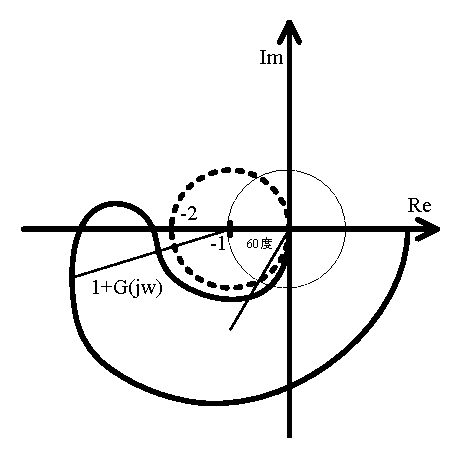
\epsfig{file=sfigure/nyquist.eps,scale=0.6}
  \caption{最適制御のナイキスト軌跡}
  \label{fig:nyquist}
 \end{center}
\end{minipage}
\ \ \ 
\begin{minipage}[c]{5cm}
 \begin{center}
　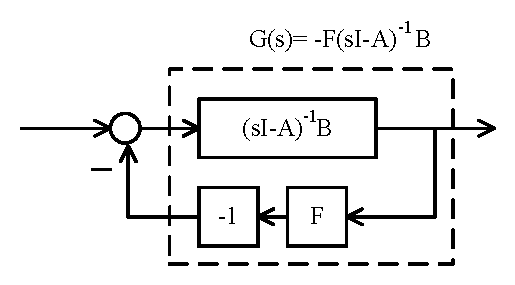
\epsfig{file=sfigure/nyquist_block.eps,scale=0.6}
  \caption{最適制御の一巡伝達関数}
  \label{fig:nyquist_block}
 \end{center}
\end{minipage}
 \end{center}
\end{figure}

\end{frame}

%%%%%%%%%%%%%%%%%%%%%%%%%%%%%%%%%%%%%%%%%%%%%%%%%%%%%%%%%%%%%%%
\begin{frame}[t]
\frametitle{2.3.4 最適制御の安定余裕（証明）}
%-------------------------------------------------------------
また，Fig.~\ref{fig:nyquist_block}のように$G(s)= - F (sI - A)^{-1} B$は閉ループ系の一巡伝達関数であるから，$G(s)$のナイキスト軌跡は最大60度位相がずれても$-1+j0$を回らない（位相余裕60度以上），
\\[3mm]

また，ゲインが$\infty$倍されても$G(s)$のナイキスト軌跡は$-1+j0$を回らない．
\\[3mm]

最悪，ナイキスト軌跡が$-1+j0$となる可能性があるのは$G(s)$のゲインが$1/2$倍より小さくなったときである．
\\[3mm]

このように最適制御は一巡伝達関数の安定余裕の意味でも良い制御系であることがわかる．

\end{frame}

%%%%%%%%%%%%%%%%%%%%%%%%%%%%%%%%%%%%%%%%%%%%%%%%%%%%%%%%%%%%%%%
\begin{frame}[t]
\frametitle{2.3.5 最適制御の漸近特性}
%-------------------------------------------------------------

\subsection{最適制御の漸近特性}

最適制御されたシステムの極と$Q$, $R$の間には次のような漸近的性質があることが知られている．これは$R$を大きく（入力に対する重みを大きくする＝入力を使わないようにする）ときと, $R$を小さくする（入力に対する重みを小さくする＝入力をどんどん使ってよい）場合に閉ループの極がどのような配置になるかを示しているものである．
\end{frame}

%%%%%%%%%%%%%%%%%%%%%%%%%%%%%%%%%%%%%%%%%%%%%%%%%%%%%%%%%%%%%%%
\begin{frame}[t]
\frametitle{2.3.5 最適制御の漸近特性}
%-------------------------------------------------------------

\begin{quote}
〔性質〕 $A$の固有値のうち安定なものを$\lambda^s_i$ $(i=1,2,\cdots,r)$, $\mbox{Re}(\lambda^s_i) < 0$，不安定なものを$\lambda^u_j$ $(j=r+1,r+2,\cdots,n)$, $\mbox{Re}(\lambda^u_j) > 0$とする．
\\{}
\ \ 
$R \rightarrow \infty$のとき(入力を極力使わないような制御をしたい場合)には，最適制御の閉ループの極は$\lambda^s_i$ $(i=1,2,\cdots,r)$($A$の安定固有値)と $-\lambda^u_j$ $(j=r+1,r+2,\cdots,n)$(虚軸に対する$A$の不安定固有値の鏡像)に収束する．

\end{quote}

\end{frame}

%%%%%%%%%%%%%%%%%%%%%%%%%%%%%%%%%%%%%%%%%%%%%%%%%%%%%%%%%%%%%%%
\begin{frame}[t]
\frametitle{2.3.5 最適制御の漸近特性}
%-------------------------------------------------------------
\small

\begin{quote}
〔性質〕 $ \mbox{det} \{G_h(-s)^T G_h(s)\}= \mbox{det}\{B^T (-sI - A^T)^{-1}H^T H (sI - A)^{-1} B\}$, ($Q=H^T H$)の零点のうち安定なものを$\sigma^s_i$ $(i=1,2,\cdots,l)$, $\mbox{Re}(\sigma^s_i) < 0$，不安定なものを$\sigma^u_j$ $(j=l+1,l+2,\cdots,2l)$, $\mbox{Re}(\sigma^u_j) > 0$とする．$ \mbox{det} \{G_h(-\sigma)^T G_h(\sigma)\}=0$ならば$ \mbox{det} \{G_h(\sigma)^T G_h(-\sigma)\}=0$となるから$\sigma^s_i=-\sigma^u_i$と仮定できる．また，$ \mbox{det} \{G_h(-s)^T G_h(s)\}$の相対次数を$2\nu=2n-2l$とする．(１入力系の場合には$ \mbox{det} \{G_h(-s)^T G_h(s)\} = G_h(-s)^T G_h(s)$である)．
\\{}
\ \ 
$R \rightarrow 0$のとき(入力をいっぱい使える場合)には，最適制御の閉ループの極は$ \mbox{det} \{G_h(\sigma)^T G_h(-\sigma)\}$の安定零点$\sigma^s_i\ (i=1,2,\cdots, l)$に収束するものと，$\nu=n-l$個の絶対値無限大に発散するもの（$s^{2\nu}+\rho \cdot (-1)^\nu=0,\  \rho \rightarrow \infty$の解のうち安定なもの，バターワースフィルタの極配置(Fig.\ref{fig:butterworth})と同じ）からなる．
\end{quote}

\begin{figure}[htbp]
 \begin{center}
　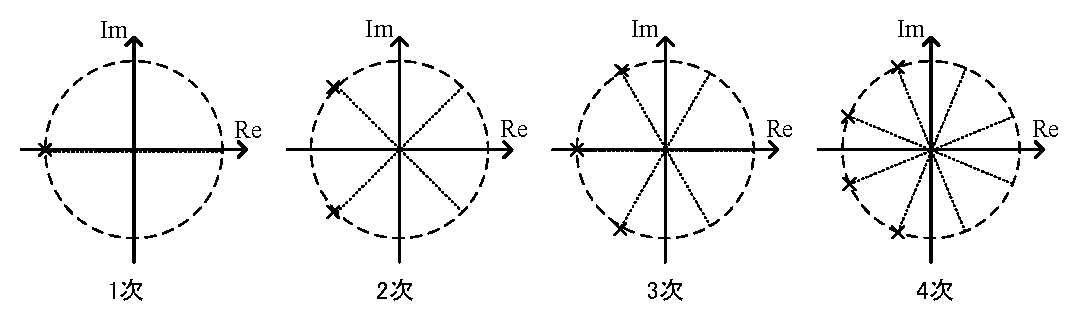
\epsfig{file=sfigure/butterworth.eps,scale=0.6}
  \caption{バターワースフィルタの極配置}
  \label{fig:butterworth}
 \end{center}
\end{figure}


\end{frame}

%%%%%%%%%%%%%%%%%%%%%%%%%%%%%%%%%%%%%%%%%%%%%%%%%%%%%%%%%%%%%%%
\begin{frame}[t]
\frametitle{2.3.5 最適制御の漸近特性}
%-------------------------------------------------------------
これらは次のように証明することができる．まず，以下の関係は行列の右辺を計算すれば証明できる．
\begin{align}
	\left(\begin{array}{cc}
		A & B \\
		C & D
	\end{array}\right)
	=
	\left(\begin{array}{cc}
		A & 0 \\
		0 & I
	\end{array}\right)
	\left(\begin{array}{cc}
		I & 0 \\
		C & D-C A^{-1}B
	\end{array}\right)
	\left(\begin{array}{cc}
		I & A^{-1}B \\
		0 & I
	\end{array}\right)
\nonumber
\end{align}
\begin{align}
	\left(\begin{array}{cc}
		A & B \\
		C & D
	\end{array}\right)
	=
	\left(\begin{array}{cc}
		I & 0 \\
		0 & D
	\end{array}\right)
	\left(\begin{array}{cc}
		A - B D^{-1} C & B \\
		0              & I
	\end{array}\right)
	\left(\begin{array}{cc}
		I        & 0 \\
		D^{-1} C & I
	\end{array}\right)
\nonumber
\end{align}
\end{frame}

%%%%%%%%%%%%%%%%%%%%%%%%%%%%%%%%%%%%%%%%%%%%%%%%%%%%%%%%%%%%%%%
\begin{frame}[t]
\frametitle{2.3.5 最適制御の漸近特性}
%-------------------------------------------------------------
行列式については$\mbox{det}(AB) = \mbox{det}(A)\mbox{det}(B)$となるから，以下の関係を得る．
\begin{align}
	\mbox{det}
	\left(\begin{array}{cc}
		A & B \\
		C & D
	\end{array}\right)
	=
	\mbox{det}A \ \mbox{det}(D-CA^{-1}B)
	=
	\mbox{det}D \ \mbox{det}({A-BD^{-1}C})	
\nonumber
\end{align}
これを用いれば以下を得る．
\begin{align}
	\mbox{det}
	\left(\begin{array}{cc}
		sI-A & B \\
		F    & I
	\end{array}\right)
	&=
	\mbox{det}(sI-A) \ \mbox{det}(I- F(sI-A)^{-1}B)
\nonumber \\
	&=
	\mbox{det}I \ \mbox{det}({sI-A - B I^{-1}F})	
	=
	\mbox{det}({sI-(A + B F)})	
\nonumber
\end{align}
\end{frame}

%%%%%%%%%%%%%%%%%%%%%%%%%%%%%%%%%%%%%%%%%%%%%%%%%%%%%%%%%%%%%%%
\begin{frame}[t]
\frametitle{2.3.5 最適制御の漸近特性}
%-------------------------------------------------------------
つまり，以下を得る．
\begin{align}
	\mbox{det}({sI-(A + B F)})	
	=
	\mbox{det}(sI-A) \ \mbox{det}(I- F(sI-A)^{-1}B)
\end{align}
同様に以下が得られる．
\begin{align}
	\mbox{det}({-sI-(A + B F)})	
	=
	\mbox{det}(-sI-A) \ \mbox{det}(I- F(-sI-A)^{-1}B)
\end{align}
\end{frame}

%%%%%%%%%%%%%%%%%%%%%%%%%%%%%%%%%%%%%%%%%%%%%%%%%%%%%%%%%%%%%%%
\begin{frame}[t]
\frametitle{2.3.5 最適制御の漸近特性}
%-------------------------------------------------------------
これを用いて
\begin{align}
	\mbox{det}R \ \mbox{det}({sI-(A + B F)})\mbox{det}({-sI-(A + B F)})
\nonumber
\end{align}
を計算すれば
\begin{align}
	& %\hspace{-1cm}
	\mbox{det}R \ \mbox{det}({sI-(A + B F)})\mbox{det}({-sI-(A + B F)})
\nonumber \\
		&= \mbox{det}R \ \mbox{det}(sI-A) \ \mbox{det}(I- F(sI-A)^{-1}B)
\nonumber \\
		&\hspace{2cm} \times
			\ \mbox{det}(-sI-A) \ \mbox{det}(I- F(-sI-A)^{-1}B)
\nonumber \\
		&= \mbox{det}(sI-A) \ \mbox{det}(-sI-A) \ 
\nonumber \\
		&\hspace{2cm} \times
			\mbox{det}(I- F(sI-A)^{-1}B) \ \mbox{det}R \ \mbox{det}(I- F(-sI-A)^{-1}B)
\end{align}
\end{frame}

%%%%%%%%%%%%%%%%%%%%%%%%%%%%%%%%%%%%%%%%%%%%%%%%%%%%%%%%%%%%%%%
\begin{frame}[t]
\frametitle{2.3.5 最適制御の漸近特性}
%-------------------------------------------------------------
ここで(\ref{kalman_eq})を用いれば次を得る．
\begin{align}
	&
	\mbox{det}R \ \mbox{det}({sI-(A + B F)})\mbox{det}({-sI-(A + B F)})
\nonumber \\
		&= \mbox{det}(sI-A) \ \mbox{det}(-sI-A) \ 
			\mbox{det}(R + B^T (-sI - A^T)^{-1}H^T H (sI - A)^{-1} B)
\label{riccati_r_q}
\end{align}
\ \\
\end{frame}

%%%%%%%%%%%%%%%%%%%%%%%%%%%%%%%%%%%%%%%%%%%%%%%%%%%%%%%%%%%%%%%
\begin{frame}[t]
\frametitle{2.3.5 最適制御の漸近特性}
%-------------------------------------------------------------
＜$R \rightarrow \infty$の場合＞

このときには(\ref{riccati_r_q})は
\begin{align}
	& %\hspace{-1cm}
	\mbox{det}R \ \mbox{det}({sI-(A + B F)})\mbox{det}({-sI-(A + B F)})
\nonumber \\
		&\hspace{2cm}
			= \mbox{det}(sI-A) \ \mbox{det}(-sI-A) \ 
			\mbox{det} R
\end{align}
と近似できる．両辺を$\mbox{det}(R )$で割れば
\begin{align}
	\mbox{det}({sI-(A + B F)})\mbox{det}({-sI-(A + B F)})
		&= \mbox{det}(sI-A) \ \mbox{det}(-sI-A) \ 
\end{align}
を得る．
\end{frame}

%%%%%%%%%%%%%%%%%%%%%%%%%%%%%%%%%%%%%%%%%%%%%%%%%%%%%%%%%%%%%%%
\begin{frame}[t]
\frametitle{2.3.5 最適制御の漸近特性}
%-------------------------------------------------------------
ここで
\begin{align}
	\mbox{det}({sI-(A + B F)})=0
\nonumber
\end{align}
の解を$s= \lambda^f_k$, $k=1,2,\cdots,n$とすると，これは閉ループ系の極であり，安定となる．また，明らかに
\begin{align}
	\mbox{det}({-sI-(A + B F)})=0
\nonumber
\end{align}
の解は$s= -\lambda^f_k$, $k=1,2,\cdots,n$となり，不安定となる．
\end{frame}

%%%%%%%%%%%%%%%%%%%%%%%%%%%%%%%%%%%%%%%%%%%%%%%%%%%%%%%%%%%%%%%
\begin{frame}[t]
\frametitle{2.3.5 最適制御の漸近特性}
%-------------------------------------------------------------
これより
\begin{align}
	\mbox{det}({sI-(A + B F)})\mbox{det}({-sI-(A + B F)})=0
\end{align}
の解は$ s= \pm \lambda^f_k$, $k=1,2,\cdots,n$となる．同様に
\begin{align}
		 \mbox{det}(sI-A) \ \mbox{det}(-sI-A) =0
\nonumber 
\end{align}
の解は$A$と$-A$の固有値と一致するため，先の定義を用いて$ s= \pm \lambda^s_i, \ \pm \lambda^u_j$, $i=1,2,\cdots,r$, $j=r+1,r+2, \cdots, n$となる．
\begin{align}
	\mbox{det}({sI-(A + B F)})\mbox{det}({-sI-(A + B F)})
		= \mbox{det}(sI-A) \ \mbox{det}(-sI-A) =0 
\nonumber 
\end{align}
を考えれば，集合として$ \{\pm \lambda^f_k\} = \{\pm \lambda^s_i, \pm \lambda^u_j\} $は等しくなる．最適制御の閉ループ極$\{\lambda^f_k\}$は安定であるから$\{\pm \lambda^s_i, \pm \lambda^u_j\} $の安定な固有値，つまり$\{\lambda^s_i, -\lambda^u_j\} $と一致する．

\ \\\
\end{frame}

%%%%%%%%%%%%%%%%%%%%%%%%%%%%%%%%%%%%%%%%%%%%%%%%%%%%%%%%%%%%%%%
\begin{frame}[t]
\frametitle{2.3.5 最適制御の漸近特性}
%-------------------------------------------------------------
＜$R \rightarrow 0$の場合＞

このときには(\ref{riccati_r_q})は
\begin{align}
	& %\hspace{-1cm}
	\mbox{det}R \ \mbox{det}({sI-(A + B F)})\mbox{det}({-sI-(A + B F)})
\nonumber \\
		&= \mbox{det}(sI-A) \ \mbox{det}(-sI-A) \ 
			\mbox{det}( B^T (-sI - A^T)^{-1}H^T H (sI - A)^{-1} B)
\end{align}
と近似される．
\end{frame}

%%%%%%%%%%%%%%%%%%%%%%%%%%%%%%%%%%%%%%%%%%%%%%%%%%%%%%%%%%%%%%%
\begin{frame}[t]
\frametitle{2.3.5 最適制御の漸近特性}
%-------------------------------------------------------------
$M^{-1}=\frac{\mbox{adj}(M)}{\mbox{det}(M)}$とあらわされることを用いれば
\begin{align}
	& %\hspace{-1cm}
	\mbox{det}R \ \mbox{det}({sI-(A + B F)})\mbox{det}({-sI-(A + B F)})
\nonumber \\
		&= \mbox{det}(sI-A) \ \mbox{det}(-sI-A) \ 
			\mbox{det}\left \{ \frac{B^T \mbox{adj}(-sI - A^T)H^T}{\mbox{det}(-sI-A)}
								\ \frac{H \mbox{adj}(sI - A) B)}{\mbox{det}(sI-A)}  \right \}
\nonumber \\
		&= \mbox{det}\left \{ {B^T \mbox{adj}(-sI - A^T)H^T} {H \mbox{adj}(sI - A) B)} \right \}
\end{align}
となり，
\end{frame}

%%%%%%%%%%%%%%%%%%%%%%%%%%%%%%%%%%%%%%%%%%%%%%%%%%%%%%%%%%%%%%%
\begin{frame}[t]
\frametitle{2.3.5 最適制御の漸近特性}
%-------------------------------------------------------------
\begin{align}
	\mbox{det}({sI-(A + B F)})\mbox{det}({-sI-(A + B F)})=0
\nonumber
\end{align}
の有界な解は
\begin{align}
	\mbox{det}\left \{ {B^T \mbox{adj}(-sI - A^T)H^T} {H \mbox{adj}(sI - A) B)} \right \}=0
\nonumber
\end{align}
の解と一致する．これは$\mbox{det}( B^T (-sI - A^T)^{-1}H^T H (sI - A)^{-1} B)$の零点に一致する．無限遠の解は根軌跡と同様に求められるが，ここでは省略する．


\end{frame}

%%%%%%%%%%%%%%%%%%%%%%%%%%%%%%%%%%%%%%%%%%%%%%%%%%%%%%%%%%%%%%%
\begin{frame}[t]
\frametitle{2.3.6 Riccati方程式の解法}
%-------------------------------------------------------------
\subsection{Riccati方程式の解法}

Riccati方程式の解法としては，数値的に安定な以下の有本-Potterの方法がよく用
いられる．まず行列$\Phi$を次のように定義する．
\begin{align}
 \Phi = \left(\begin{array}{cc}
	       A  & - B R^{-1} B^T \\
	       -Q & - A^T
	      \end{array}\right)
\end{align}
\end{frame}

%%%%%%%%%%%%%%%%%%%%%%%%%%%%%%%%%%%%%%%%%%%%%%%%%%%%%%%%%%%%%%%
\begin{frame}[t]
\frametitle{2.3.6 Riccati方程式の解法(有本-Potterの方法)}
%-------------------------------------------------------------
この$\Phi$の固有値のうち実部が負のものが$n$個あることが分かっている．これらの固有値を$\lambda_i$, $i=1,2,\cdots,n$とし，これに対応する固有ベクトルを$w_1, w_2, \cdots, w_n$する．この固有ベクトルを次のように分解しておく．
\begin{align}
 w_i = \left(\begin{array}{c}
	      \xi_i \\
	      \eta_i
	     \end{array}\right), \hspace{1cm} \xi_i \in {\mathbb R}^n, \ \eta_i \in {\mathbb R}^n
\end{align}
このとき
\begin{align}
	P = Y X^{-1}, \ \ \ 
	X = (\xi_1, \xi_2, \cdots, \xi_n), \ \ \ 
	Y = (\eta_1, \eta_2, \cdots, \eta_n)
\end{align}
と選べば$P$は正定かつRiccati方程式を満たすことが知られている．
\end{frame}

%%%%%%%%%%%%%%%%%%%%%%%%%%%%%%%%%%%%%%%%%%%%%%%%%%%%%%%%%%%%%%%
\begin{frame}[t]
\frametitle{2.3.6 Riccati方程式の解法(有本-Potterの方法:証明)}
%-------------------------------------------------------------

これを証明しよう．まず，$\lambda$が$\Phi$の固有値であるとき，$-\lambda$も固有値であることが次のように証明できる．\\[3mm]

まず，$\lambda$と$w = (\xi^T, \eta^T)^T$が固有値と固有ベクトルであるとすると
\begin{align}
	\left(\begin{array}{cc}
	       A  & - B R^{-1} B^T \\
	       -Q & - A^T
	\end{array}\right)
		  \left(\begin{array}{c}
	        \xi \\
	        \eta
	      \end{array}\right)
	&= \lambda
		  \left(\begin{array}{c}
	        \xi \\
	        \eta
	      \end{array}\right)
\nonumber \\
	\left(\begin{array}{c}
	       A \xi - B R^{-1} B^T \eta \\
	       -Q\xi - A^T \eta
	\end{array}\right)
	&=
		  \left(\begin{array}{c}
	        \lambda \xi \\
	        \lambda \eta
	      \end{array}\right)
\label{potter_1}
\end{align}
を得る．
\end{frame}

%%%%%%%%%%%%%%%%%%%%%%%%%%%%%%%%%%%%%%%%%%%%%%%%%%%%%%%%%%%%%%%
\begin{frame}[t]
\frametitle{2.3.6 Riccati方程式の解法(有本-Potterの方法:証明)}
%-------------------------------------------------------------
次に
\begin{align}
	\Phi^T 
		  \left(\begin{array}{c}
	        - \eta \\
	          \xi
	      \end{array}\right)
\nonumber	
\end{align}
を計算すれば
\begin{align}
	\Phi^T 
		  \left(\begin{array}{c}
	        - \eta \\
	          \xi
	      \end{array}\right)
	&=
	\left(\begin{array}{cc}
	       A^T            &  -Q \\
	       - B R^{-1} B^T & - A
	\end{array}\right)
		  \left(\begin{array}{c}
	        - \eta \\
	          \xi
	      \end{array}\right)
	=
	\left(\begin{array}{c}
	       - A^T \eta  -Q \xi \\
	       B R^{-1} B^T \eta - A \xi
	\end{array}\right)
\end{align}
となる．
\end{frame}

%%%%%%%%%%%%%%%%%%%%%%%%%%%%%%%%%%%%%%%%%%%%%%%%%%%%%%%%%%%%%%%
\begin{frame}[t]
\frametitle{2.3.6 Riccati方程式の解法(有本-Potterの方法:証明)}
%-------------------------------------------------------------
ここで(\ref{potter_1})を用いれば
\begin{align}
	\Phi^T 
		  \left(\begin{array}{c}
	        - \eta \\
	          \xi
	      \end{array}\right)
	&=
		  \left(\begin{array}{c}
	        \lambda \eta \\
	        - \lambda \xi
	      \end{array}\right)
	= -\lambda
		  \left(\begin{array}{c}
	        -\eta \\
	        \xi
	      \end{array}\right)
\end{align}
となり，$-\lambda$が$\Phi^T$の固有値となる．
\\[3mm]

$\Phi$と$\Phi^T$の固有値は一致するから，$-\lambda$も$\Phi$の固有値となる．
\\[3mm]

つまり，$2n \times 2n$の行列$\Phi$は$n$個の安定固有値と$n$個の不安定固有値を持つことになる．（虚軸上に極を持たない証明は省略する）

\end{frame}

%%%%%%%%%%%%%%%%%%%%%%%%%%%%%%%%%%%%%%%%%%%%%%%%%%%%%%%%%%%%%%%
\begin{frame}[t]
\frametitle{2.3.6 Riccati方程式の解法(有本-Potterの方法:証明)}
%-------------------------------------------------------------
さて，安定固有値と対応する固有ベクトルを先の定義のように選ぶと次が成り立つ．
\begin{align}
	\left(\begin{array}{cc}
	       A  & - B R^{-1} B^T \\
	       -Q & - A^T
	\end{array}\right)
		 \left(\begin{array}{c}
		      X \\
		      Y
		\end{array}\right)
	= 
		 \left(\begin{array}{cccc}
		      X \\
		      Y
		\end{array}\right)
		\Lambda
		, \ \ \ 
		\Lambda =
		 \left(\begin{array}{cccc}
		      \lambda_1 & & &  \\
		      & \lambda_2 & &  \\
		      & & \ddots    &  \\
		      & & & \lambda_n 
		\end{array}\right)
\end{align}
\end{frame}

%%%%%%%%%%%%%%%%%%%%%%%%%%%%%%%%%%%%%%%%%%%%%%%%%%%%%%%%%%%%%%%
\begin{frame}[t]
\frametitle{2.3.6 Riccati方程式の解法(有本-Potterの方法:証明)}
%-------------------------------------------------------------
この両辺に$X^{-1}$を右から乗じて整理すると($X^{-1}X =I$を右辺に挿入している)
\begin{align}
	\left(\begin{array}{cc}
	       A  & - B R^{-1} B^T \\
	       -Q & - A^T
	\end{array}\right)
		 \left(\begin{array}{c}
		      X \\
		      Y
		\end{array}\right)
		X^{-1}
	&= 
		 \left(\begin{array}{cccc}
		      X \\
		      Y
		\end{array}\right)
		X^{-1} X \Lambda
		X^{-1}
\nonumber \\
	\left(\begin{array}{cc}
	       A  & - B R^{-1} B^T \\
	       -Q & - A^T
	\end{array}\right)
		 \left(\begin{array}{c}
		      I \\
		      YX^{-1}
		\end{array}\right)
	&= 
		 \left(\begin{array}{cccc}
		      I \\
		      YX^{-1}
		\end{array}\right)
		X \Lambda
		X^{-1}
\nonumber \\
	\left(\begin{array}{cc}
	       A  & - B R^{-1} B^T \\
	       -Q & - A^T
	\end{array}\right)
		 \left(\begin{array}{c}
		      I \\
		      P
		\end{array}\right)
	&= 
		 \left(\begin{array}{cccc}
		      I \\
		      P
		\end{array}\right)
		\bar{\Lambda}
		, \ \ \ 
		\bar{\Lambda} = X \Lambda X^{-1}
\end{align}
となる．（$P$の正定性についてはここでは証明を省略する）．
\end{frame}

%%%%%%%%%%%%%%%%%%%%%%%%%%%%%%%%%%%%%%%%%%%%%%%%%%%%%%%%%%%%%%%
\begin{frame}[t]
\frametitle{2.3.6 Riccati方程式の解法(有本-Potterの方法:証明)}
%-------------------------------------------------------------
この左辺と右辺を計算すれば
\begin{align}
	\left(\begin{array}{cc}
	       A  & - B R^{-1} B^T \\
	       -Q & - A^T
	\end{array}\right)
		 \left(\begin{array}{c}
		      I \\
		      P
		\end{array}\right)
	&= 
	\left(\begin{array}{c}
	       A  - B R^{-1} B^T P \\
	       -Q - A^T P
	\end{array}\right)
\nonumber \\
		 \left(\begin{array}{cccc}
		      I \\
		      P
		\end{array}\right)
		\bar{\Lambda}
		& = 
		 \left(\begin{array}{cccc}
		      \bar{\Lambda} \\
		      P \bar{\Lambda}
		\end{array}\right)
\nonumber 
\end{align}
より
\begin{align}
	\left(\begin{array}{c}
	       A  - B R^{-1} B^T P \\
	       -Q - A^T P
	\end{array}\right)
		& = 
		 \left(\begin{array}{cccc}
		      \bar{\Lambda} \\
		      P \bar{\Lambda}
		\end{array}\right)
\nonumber 
\end{align}
を得る．
\end{frame}

%%%%%%%%%%%%%%%%%%%%%%%%%%%%%%%%%%%%%%%%%%%%%%%%%%%%%%%%%%%%%%%
\begin{frame}[t]
\frametitle{2.3.6 Riccati方程式の解法(有本-Potterの方法:証明)}
%-------------------------------------------------------------
つまり，
\begin{align}
	       A  - B R^{-1} B^T P & = \bar{\Lambda} 
\nonumber \\
	       -Q - A^T P & = P \bar{\Lambda}
\nonumber 
\end{align}
となる．第１式に左から$P$を乗じれば
\begin{align}
	       P A  - P B R^{-1} B^T P & = P \bar{\Lambda} 
\nonumber \\
	       -Q - A^T P & = P \bar{\Lambda}
\nonumber
\end{align}
となる．右辺が等しいことから
\begin{align}
	       P A  - P B R^{-1} B^T P = -Q - A^T P
\nonumber
\end{align}
となり，これを変形するとRiccati方程式となる．
\end{frame}

%%%%%%%%%%%%%%%%%%%%%%%%%%%%%%%%%%%%%%%%%%%%%%%%%%%%%%%%%%%%%%%
\begin{frame}[t]
\frametitle{2.3.6 Riccati方程式の解法(有本-Potterの方法:性質)}
%-------------------------------------------------------------
さらに最適制御の閉ループ系は$A  - B R^{-1} B^T P = \bar{\Lambda}$となっている．
\\[3mm]

$\bar{\Lambda} = X \Lambda X^{-1}$より$\bar{\Lambda}$と$\Lambda$の固有値は等しいから，$\Phi$の安定固有値が閉ループ系の極と一致することにも注意する．\\

\end{frame}

%%%%%%%%%%%%%%%%%%%%%%%%%%%%%%%%%%%%%%%%%%%%%%%%%%%%%%%%%%%%%%%
\begin{frame}[t]
\frametitle{2.3.6 Riccati方程式の解法(演習)}
%-------------------------------------------------------------
\noindent
{\bf [演習]}\nopagebreak
次の最適制御問題を考える．
\begin{align}
	\frac{dx}{dt} & = 1 \cdot x + 1 \cdot u
\nonumber \\
	J &= \int q x^2 + r u^2 dt
\end{align}
$q=1$として以下を求めよ．
\begin{description}
  \item[1.]  最適フィードバックをRiccati方程式(２次方程式)を直接解くことにより求めよ．
  \item[2.]  フィードバック系の状態方程式を求めよ．
  \item[3.]  フィードバック系の極を求めよ．
  \item[4.]  $r \rightarrow 0$の場合にフィードバック系の極がどこに漸近するかを示せ．
  \item[5.]  $r \rightarrow \infty$の場合にフィードバック系の極がどこに漸近するかを示せ．
\end{description}

\noindent
{\bf [演習]}\nopagebreak
上記演習のRiccati方程式を有本-Potterの方法を用いて解け．

\end{frame}

%%%%%%%%%%%%%%%%%%%%%%%%%%%%%%%%%%%%%%%%%%%%%%%%%%%%%%%%%%%%%%%
\begin{frame}[t]
\frametitle{2.4.1 外乱オブザーバ}
%-------------------------------------------------------------
%..........................................................

\section{オブザーバ：最小次元オブザーバと外乱オブザーバ}



\subsection{外乱オブザーバー}
%---------------------------------------------------------------------------
システムに未知の定数外乱がある場合には，オブザーバーが状態の推定器として十分に
動作しないことがある．このような場合には外乱まで推定するようなオブザーバーを
作ってしまう方法がある．
\\[3mm]

次のようなシステムを考える．
\begin{align}
 \frac{dx}{dt} &= A x + B u + E \delta \nonumber \\
 y             &= C x
\end{align}
ここで$\delta$は外乱であり，未知ではあるが一定値(またはゆっくり変化する)と
仮定する．
\end{frame}

%%%%%%%%%%%%%%%%%%%%%%%%%%%%%%%%%%%%%%%%%%%%%%%%%%%%%%%%%%%%%%%
\begin{frame}[t]
\frametitle{2.4.1 外乱オブザーバ}
%-------------------------------------------------------------
このシステムに通常の方法でオブザーバーを
\begin{equation}
 \frac{d \hat{x}}{dt} = A \hat{x} + B u - K(y - C \hat{x})
\end{equation}
とすると，推定誤差$e = x - \hat{x}$は
\begin{align}
 \frac{de}{dt} &= \frac{dx}{dt} - \frac{d\hat{x}}{dt} \nonumber \\
 &= Ax + Bu + E \delta - A\hat{x} - Bu + K(y - C \hat{x}) \nonumber \\
 &= Ax + Bu + E \delta - A\hat{x} - Bu + K(Cx - C \hat{x}) \nonumber  \\
 &= (A+KC)(x-\hat{x}) + E \delta \nonumber \\
 &= (A+KC)e + E \delta
\end{align}
となり，$e$は$\delta$の影響により$0$に収束しなくなり，$\hat{x}$は$x$に対して
常に偏差を持ってしまう（ただし，フィードバック系の安定性に関しては問題はない）．
\end{frame}

%%%%%%%%%%%%%%%%%%%%%%%%%%%%%%%%%%%%%%%%%%%%%%%%%%%%%%%%%%%%%%%
\begin{frame}[t]
\frametitle{2.4.1 外乱オブザーバ}
%-------------------------------------------------------------
このような場合にも，偏差を持たない状態の推定値が必要なときには外乱$\delta$まで推定してしまえばよい．
\\[3mm]

いま，$\delta$は未知ではあるが一定値であるから
\begin{equation}
 \frac{d \delta}{dt} = 0
\end{equation}
と表すことが出来る．これを用いて元のシステムを$x$と$\delta$を状態とする拡大
系として表せば
\begin{align}
 \frac{d}{dt}
  \left(\begin{array}{c}
         x \\
	 \delta
	\end{array}\right)
  &=
  \left(\begin{array}{cc}
         A & E \\
	 0 & 0
	\end{array}\right)
  \left(\begin{array}{c}
         x \\
	 \delta
	\end{array}\right)
  +
  \left(\begin{array}{c}
         B \\
	 0
	\end{array}\right)
  u \\
 y &=
  \left(\begin{array}{cc}
         C & 0
	\end{array}\right) 
  \left(\begin{array}{c}
	 x \\
	 \delta
	\end{array}\right)
\end{align}
となる．
\end{frame}

%%%%%%%%%%%%%%%%%%%%%%%%%%%%%%%%%%%%%%%%%%%%%%%%%%%%%%%%%%%%%%%
\begin{frame}[t]
\frametitle{2.4.1 外乱オブザーバ}
%-------------------------------------------------------------
このシステムのオブザーバーとして
\begin{align}
 \frac{d}{dt}
  \left(\begin{array}{c}
         \hat{x} \\
	 \hat{\delta}
	\end{array}\right)
  &=
  \left(\begin{array}{cc}
         A & E \\
	 0 & 0
	\end{array}\right)
  \left(\begin{array}{c}
         \hat{x} \\
	 \hat{\delta}
	\end{array}\right)
  +
  \left(\begin{array}{c}
         B \\
	 0
	\end{array}\right)
  u -
  \left(\begin{array}{c}
         K_1 \\
	 K_2
	\end{array}\right)
  \left[y -
   \left(\begin{array}{cc}
          C & 0
	 \end{array}\right)
   \left(\begin{array}{c}
	  \hat{x} \\
	  \hat{\delta}
	 \end{array}\right)\right] \nonumber \\
\end{align}
を設計すれば，状態$x$とともに外乱$\delta$も同時に誤差なく推定できる．
\\[3mm]

このオブザーバーは外乱が存在する場合の状態推定としてのみではなく，外乱の検出器としても用いることが出来る(外乱が一定でなくてもゆっくり変化する場合にも使うことが出来る)．
\\[3mm]

例えば，ロボット制御で力を外乱と考え，高価な力センサーの代わりに力検出器として用いた例もある．

\end{frame}

%%%%%%%%%%%%%%%%%%%%%%%%%%%%%%%%%%%%%%%%%%%%%%%%%%%%%%%%%%%%%%%
\begin{frame}[t]
\frametitle{2.4.1 外乱オブザーバ}
%-------------------------------------------------------------
この外乱オブザーバーは別の用途に使うこともできる．
\\[3mm]

いま$B=E$の場合,つまり
\begin{equation}
 \frac{dx}{dt} = A x + B u + B \delta
\end{equation}
の場合には，新しい入力を$v$として$u$を
\begin{equation}
 u = v - \hat{\delta}
\end{equation}
とすれば，システムは
\begin{equation}
 \frac{dx}{dt} = A x + B v + B (\delta- \hat{\delta})
\end{equation}
となり，近似的に外乱$\delta$を打ち消すことが出来る．

\end{frame}

%%%%%%%%%%%%%%%%%%%%%%%%%%%%%%%%%%%%%%%%%%%%%%%%%%%%%%%%%%%%%%%
\begin{frame}[t]
\frametitle{2.4.1 外乱オブザーバ}
%-------------------------------------------------------------
これを発展させると，システムの不確定性に対してもロバストな制御系を設計す
ることが出来る．
\\[3mm]

いま，実際のプラントが時変かつ未知の行列$\Delta(t)$を用
いて
\begin{align}
  \frac{dx}{dt} & = A_t x + B_t u + B \delta 
\\
  & A_t = A + B \Delta_1(t), \quad B_t = B + B\Delta_2(t)
\nonumber 
\end{align}
と表されていたとしよう．このときシステムを
\begin{align}
 \frac{dx}{dt}
  &= (A + B \Delta_1(t))x + (B + B\Delta_2(t)) u + B \delta \nonumber \\
 &= A x + B u + B (\Delta_1(t) x + \Delta_2(t) u +\delta) \nonumber \\
 &= Ax + Bu + B \bar{\delta(t)}
\end{align}
とシステムの誤差$\Delta(t)$を仮想的な外乱$\bar{\delta}$と考え，これが十分ゆ
っくり変化すると仮定し，外乱として推定することで，先ほどの方法で打ち消す
方法がある．これは特にモーター系などに有効であることがわかっている．
%---------------------------------------------------------------------------




\end{frame}


%%%%%%%%%%%%%%%%%%%%%%%%%%%%%%%%%%%%%%%%%%%%%%%%%%%%%%%%%%%%%%%
\begin{frame}[t]
\frametitle{2.4.2 最小次元オブザーバ}
%-------------------------------------------------------------
\subsection{最小次元オブザーバ}

今までのオブザーバは状態$x$をすべて推定したが，ここでは状態の一部を推定することを考える．
次のシステムを考える．
\begin{align}
 \frac{dx}{dt} &= A x + B u  \nonumber \\
 y             &= C x \ \ \ \in R^p
\end{align}
いま状態$x$の線形関数$z=Ux \in R^{n-p}$を考える．このとき出力$y= Cx$を用いれば
\begin{equation}
   \left(\begin{array}{c}
	z \\
	y
   \end{array}\right)
   =
   \left(\begin{array}{c}
	U \\
	C
   \end{array}\right)
   x
\end{equation}
となる．
\end{frame}

%%%%%%%%%%%%%%%%%%%%%%%%%%%%%%%%%%%%%%%%%%%%%%%%%%%%%%%%%%%%%%%
\begin{frame}[t]
\frametitle{2.4.2 最小次元オブザーバ}
%-------------------------------------------------------------
いま
\begin{equation}
   \left(\begin{array}{c}
	U \\
	C
   \end{array}\right)
\end{equation}
が正則になるように$U$を選べば
\begin{equation}
   \left(\begin{array}{c}
	U \\
	C
   \end{array}\right) ^{-1}
   \left(\begin{array}{c}
	z \\
	y
   \end{array}\right)
   =
   x
\end{equation}
となり，$y$と$z$より状態$x$が得られることになる．
\end{frame}

%%%%%%%%%%%%%%%%%%%%%%%%%%%%%%%%%%%%%%%%%%%%%%%%%%%%%%%%%%%%%%%
\begin{frame}[t]
\frametitle{2.4.2 最小次元オブザーバ}
%-------------------------------------------------------------
さてこのような$z=Ux$の推定値$\hat{z}$を次のシステムで求めることを考える．
\begin{equation}
   \frac{d\hat{z}}{dt} = \hat{A} \hat{z} + \hat{B} y + \hat{J} u
\end{equation}
$z=Ux$と$\hat{z}$の差を
\begin{equation}
   \zeta = z - \hat{z} = Ux -\hat{z}
\end{equation}
と定義すれば
\begin{eqnarray}
   \frac{d \zeta}{dt} & = & U \frac{dx}{dt} - \frac{d \hat{z}}{dt}
\nonumber \\
   & = & U A x + U B u - \hat{A} \hat{z} - \hat{B} y - \hat{J} u
\nonumber \\
   & = & U A x + U B u - \hat{A} \hat{z} - \hat{B} y - \hat{J} u +\hat{A}Ux - \hat{A}Ux \hspace{0.4cm} \mbox{($\hat{A}Ux$を足して引く)}
\nonumber \\
   & = & \hat{A}( Ux - \hat{z} ) + ( U B - \hat{J} ) u 
	 + ( U A - \hat{A} U - \hat{B} C ) x
\nonumber \\
   & = & \hat{A} \zeta + ( U B - \hat{J} ) u 
	 + ( U A - \hat{A} U - \hat{B} C ) x
\end{eqnarray}
\end{frame}

%%%%%%%%%%%%%%%%%%%%%%%%%%%%%%%%%%%%%%%%%%%%%%%%%%%%%%%%%%%%%%%
\begin{frame}[t]
\frametitle{2.4.2 最小次元オブザーバ}
%-------------------------------------------------------------
よって$\hat{A},\hat{B},\hat{J}$を
\begin{equation}
    U A - \hat{A} U - \hat{B} C = 0, 
    \ \ \ \mbox{またはブロック行列表現で}\ \ 
  {\small
   UA = 
   \left(\begin{array}{cc}
	\hat{A} & \hat{B}
   \end{array}\right)
	   \left(\begin{array}{c}
		U \\
		C
	   \end{array}\right) 
	}
\end{equation}
\begin{equation}
    U B = \hat{J}
\end{equation}
\begin{equation}
    \hat{A} : \mbox{ 安定行列}
\end{equation}
を満たすように選べば入力$u$や初期値$\hat{z}(0)$に関係なく$ \zeta \rightarrow 0 $となり$\hat{z}$が$z=Ux$の推定値となる．
\end{frame}

%%%%%%%%%%%%%%%%%%%%%%%%%%%%%%%%%%%%%%%%%%%%%%%%%%%%%%%%%%%%%%%
\begin{frame}[t]
\frametitle{2.4.2 最小次元オブザーバ}
%-------------------------------------------------------------
またこのとき$x$の推定値$\hat{x}$は
\begin{equation}
   \left(\begin{array}{cc}
	\hat{C} & \hat{D} \\
   \end{array}\right)
	\defeq \left(\begin{array}{c}
			U \\
			C 
		\end{array}\right) ^{-1}
\end{equation}
として
\begin{equation}
   \hat{x} = \hat{C} \hat{z} + \hat{D}y
\end{equation}
で表わされる．
\\[3mm]

このオブザーバの次元（$\hat{z}$の次元: $n-p$）はシステムの次元（$x$の次元: $n$）よりも小さく，またこれ以上小さい次元のシステムで状態を推定することができないことが分かっている．
\\[3mm]

そこでこのようなオブザーバを最小次元オブザーバという．
\end{frame}

%%%%%%%%%%%%%%%%%%%%%%%%%%%%%%%%%%%%%%%%%%%%%%%%%%%%%%%%%%%%%%%
\begin{frame}[t]
\frametitle{2.4.2 最小次元オブザーバ}
%-------------------------------------------------------------
以上の議論をまとめると最小次元オブザーバの満たすべき条件は以下のようになる．
\begin{eqnarray}
   \left(\begin{array}{cc}
	\hat{A} & \hat{B} \\
	\hat{C} & \hat{D}
   \end{array}\right)
   & = &   \left(\begin{array}{c}
		UA \\
		I
	   \end{array}\right)
	   \left(\begin{array}{c}
		U \\
		C
	   \end{array}\right) ^{-1}
\label{obs_cond_1} \\
   \hat{J} & = & UB
\label{obs_cond_2} \\
   \hat{A} & : & \mbox{安定}
\label{obs_cond_3}
\end{eqnarray}
となる．このとき，$U$が決まれば$\hat{A},\hat{B},\hat{C},\hat{D},\hat{J}$が決定されるので，最小次元オブザーバの設計は$U$を設計することとなる．

\end{frame}

%%%%%%%%%%%%%%%%%%%%%%%%%%%%%%%%%%%%%%%%%%%%%%%%%%%%%%%%%%%%%%%
\begin{frame}[t]
\frametitle{2.4.2 最小次元オブザーバ(Gopinathのアルゴリズム)}
%-------------------------------------------------------------
最小次元オブザーバの設計法に関しては次のGopinathのアルゴリズムがよく知られている．

\noindent \underline{step.1}
次の行列が正則になるような行列$C^*$を選ぶ．
\begin{equation}
	\left(\begin{array}{c}
		C^* \\ 
		C 
	\end{array}\right)
\end{equation}

\end{frame}

%%%%%%%%%%%%%%%%%%%%%%%%%%%%%%%%%%%%%%%%%%%%%%%%%%%%%%%%%%%%%%%
\begin{frame}[t]
\frametitle{2.4.2 最小次元オブザーバ(Gopinathのアルゴリズム)}
%-------------------------------------------------------------
\noindent \underline{step.2}
座標変換行列$T$を
\begin{equation}
        T =
	\left(\begin{array}{c}
		C^* \\ 
		C 
	\end{array}\right) ^{-1}
\end{equation}
とし，システムを座標変換し，以下の行列を得る．($I_k$は${\mathbb R}^{(k \times k)}$の単位行列)
\begin{eqnarray}
   \bar{A} & = & T^{-1} A T = \left(\begin{array}{cc}
				\bar{A}_{11} & \bar{A}_{12} \\
				\bar{A}_{21} & \bar{A}_{22} \\
			      \end{array}\right)
\\
   \bar{B} & = & T^{-1} B = \left(\begin{array} {c}
				\bar{B}_1 \\
				\bar{B}_2 
			    \end{array}\right)
\\
   \bar{C} & = & C T = \left(\begin{array}{cc}
				0 & I_{p} \\
			\end{array}\right)
\end{eqnarray}

\end{frame}

%%%%%%%%%%%%%%%%%%%%%%%%%%%%%%%%%%%%%%%%%%%%%%%%%%%%%%%%%%%%%%%
\begin{frame}[t]
\frametitle{2.4.2 最小次元オブザーバ(Gopinathのアルゴリズム)}
%-------------------------------------------------------------
\noindent \underline{step.3}
$(\bar{A}, \bar{B}, \bar{C})$のオブザーバ$(\hat{\bar{A}}, \hat{\bar{B}}, \hat{\bar{C}}, \hat{\bar{D}}, \hat{\bar{J}})$を求める．このとき次の$\bar{U}$を用いる．
\begin{equation}
   \bar{U} = \left(\begin{array}{cc}
		I_{n-p} & -L
	     \end{array}\right)
\end{equation}

ここまでのステップで
\begin{align}
	\left(\begin{array}{c}
		\bar{U} \\
		\bar{C}
	\end{array}\right)
	=
	\left(\begin{array}{cc}
		I_{n-p} & -L \\
		0 &  I_{p} 
	\end{array}\right) ^{-1}
\end{align}
となり，この逆行列が
\begin{align}
	\left(\begin{array}{c}
		\bar{U} \\
		\bar{C}
	\end{array}\right)^{-1}
	=
	\left(\begin{array}{cc}
		I_{n-p} & -L \\
		0 &  I_{p} 
	\end{array}\right) ^{-1}
	=
	\left(\begin{array}{cc}
		I_{n-p} & L \\
		0 &  I_{p} 
	\end{array}\right)
\end{align}
と単純な形になることに注意する．\\

\end{frame}

%%%%%%%%%%%%%%%%%%%%%%%%%%%%%%%%%%%%%%%%%%%%%%%%%%%%%%%%%%%%%%%
\begin{frame}[t]
\frametitle{2.4.2 最小次元オブザーバ(Gopinathのアルゴリズム)}
%-------------------------------------------------------------
\noindent \underline{step.4}
$\bar{U}$の定義より(\ref{obs_cond_1})は
\begin{eqnarray}
   \left(\begin{array}{cc}
	\hat{\bar{A}} & \hat{\bar{B}} \\
	\hat{\bar{C}} & \hat{\bar{D}}
   \end{array}\right)
   & = & 	   \left(\begin{array}{c}
		( I_{n-p}, -L) \bar{A} \\
		I_{n}
	   \end{array}\right)
	   \left(\begin{array}{cc}
		I_{n-p} & -L \\
		0 &  I_{p} 
	   \end{array}\right) ^{-1}
\nonumber \\
   & = &    \left(\begin{array}{c|c}
		\bar{A}_{11} - L \bar{A}_{21} &
			\bar{A}_{12} - L \bar{A}_{22} \\
		\hline
		I_{n-p}  & 0 \\
		0        & I_{p}
	   \end{array}\right)
	   \left(\begin{array}{cc}
		I_{n-p} & L \\
		0 &  I_{p} 
	   \end{array}\right) 
\end{eqnarray}
\end{frame}

%%%%%%%%%%%%%%%%%%%%%%%%%%%%%%%%%%%%%%%%%%%%%%%%%%%%%%%%%%%%%%%
\begin{frame}[t]
\frametitle{2.4.2 最小次元オブザーバ(Gopinathのアルゴリズム)}
%-------------------------------------------------------------
よって
\begin{eqnarray}
   \hat{\bar{A}} & = & \bar{A}_{11} - L \bar{A}_{21}
\label{temp12}
\\
   \hat{\bar{B}} & = & \bar{A}_{11} L - L \bar{A}_{21} L 
				+ \bar{A}_{12} - L \bar{A}_{22}
\\
   \hat{\bar{C}} & = & \left(\begin{array}{c}
				I_{n-p} \\
				0 
			\end{array}\right)
\\
   \hat{\bar{D}} & = & \left(\begin{array}{c}
				L  \\
				I_{p} 
			\end{array}\right)
\\
   \hat{\bar{J}} & = & \bar{U} \bar{B}
		 \ = \ \bar{B}_1 - L \bar{B}_2
\end{eqnarray}
となる．$(C,A)$可観測であるならば$(\bar{A}_{21},\bar{A}_{11})$が可観測であることが証明できる．そこで，$L$は$\hat{\bar{A}}$が安定になるように選べる．

\end{frame}

%%%%%%%%%%%%%%%%%%%%%%%%%%%%%%%%%%%%%%%%%%%%%%%%%%%%%%%%%%%%%%%
\begin{frame}[t]
\frametitle{2.4.2 最小次元オブザーバ(Gopinathのアルゴリズム)}
%-------------------------------------------------------------
\noindent \underline{step.5}
いままでは状態$\bar{x}$のオブザーバをつくってきた．$T \bar{x} = x$であるから状態$x$のオブザーバは
\begin{equation}
   \hat{A} = \hat{\bar{A}}
, \hspace{2mm}
   \hat{B} = \hat{\bar{B}}
, \hspace{2mm}
   \hat{C} = T \hat{\bar{C}}
, \hspace{2mm}
   \hat{D} = T \hat{\bar{D}}
, \hspace{2mm}
   \hat{J} = \hat{\bar{J}}
\end{equation}
で与えられる．
\end{frame}

%%%%%%%%%%%%%%%%%%%%%%%%%%%%%%%%%%%%%%%%%%%%%%%%%%%%%%%%%%%%%%%
\begin{frame}[t]
\frametitle{2.4.2 最小次元オブザーバ\\ (最小次元オブザーバの利点・欠点)}
%-------------------------------------------------------------

\subsubsection{最小次元オブザーバの利点・欠点}

最小次元オブザーバは「次元が小さいので計算量が少ない」，「出力に関する部分の推定に遅れがない」という利点がある
\\[3mm]

一方「出力の外乱の影響を直接受けるため，カルマンフィルタなどに比べて出力外乱に影響されやすい」という欠点がある．\\[3mm]

実際の利用に関してはこれらの得失を理解の上，オブザーバ手法を選ぶ必要がある．

\end{frame}

%%%%%%%%%%%%%%%%%%%%%%%%%%%%%%%%%%%%%%%%%%%%%%%%%%%%%%%%%%%%%%%
\begin{frame}[t]
\frametitle{2.5 可制御性(可到達性)・可安定性}
%-------------------------------------------------------------
\section{可制御性(可到達性)・可安定性}
%---------------------------------------------------------------------------

ここでは可制御性に関連して可到達性，可安定性などの性質について詳しく述べる．


\end{frame}

%%%%%%%%%%%%%%%%%%%%%%%%%%%%%%%%%%%%%%%%%%%%%%%%%%%%%%%%%%%%%%%
\begin{frame}[t]
\frametitle{2.5.1 可制御性の定義}
%-------------------------------------------------------------
\subsection{可制御性の定義}

状態方程式(1.1)において初期状態$x(0)=x_0$を有限時間$t_1$で原点に移す$(x(t_1)=0)$入力$u(t), t\in[0,t_1]$が存在するとき$x_0$は{\bf 可制御(controllable)}であるという．
\\[3mm]

また，すべての状態$x_0$が可制御であるとき，状態方程式は可制御であるという．
\\[3mm]

可制御でない状態方程式は{\bf 不可制御(uncontrollable)}であるという．
\\[3mm]

可制御性は$A,B$行列のみに依存する性質なので{\bf $(A,B)$可制御}ということもある．

\end{frame}

%%%%%%%%%%%%%%%%%%%%%%%%%%%%%%%%%%%%%%%%%%%%%%%%%%%%%%%%%%%%%%%
\begin{frame}[t]
\frametitle{2.5.1 可制御性の定義}
%-------------------------------------------------------------
可制御に対して{\bf 可到達(reachable)}という概念もある．
\\[3mm]

可到達なシステムとは$x(0)=0$から入力により有限時間で任意の状態へ移動可能なシステムである．
\\[3mm]

ここで考えている（線形な）状態方程式の範囲では{\bf 可制御性(controllability)}と{\bf 可到達性(reachability)}は同値な関係にある．つまり，可制御とは基本的には入力を用いて状態を制御できるということである．

\end{frame}

%%%%%%%%%%%%%%%%%%%%%%%%%%%%%%%%%%%%%%%%%%%%%%%%%%%%%%%%%%%%%%%
\begin{frame}[t]
\frametitle{2.5.1 可制御性の定義}
%-------------------------------------------------------------
可制御性と可到達性が同値であることは次のように証明できる．状態方程式の解は
\begin{align}
	x(t) = e^{At} x_0 + \int_0^t e^{A(t-\tau)} B u (\tau) d \tau
\end{align}
と表せる．いま，状態方程式が可制御であるならば，有限時間$t_1$と入力$u^*(t), t\in[0,t_1]$が存在して，$x(t_1)=0$となる．これは
\begin{align}
	0 = e^{At_1} x_0 + \int_0^{t_1} e^{A(t-\tau)} B u^* (\tau) d \tau
\end{align}
を意味している．これを変形すれば
\begin{align}
	-e^{At_1} x_0 = \int_0^{t_1} e^{A(t-\tau)} B u^* (\tau) d \tau
\end{align}
となる．
\end{frame}

%%%%%%%%%%%%%%%%%%%%%%%%%%%%%%%%%%%%%%%%%%%%%%%%%%%%%%%%%%%%%%%
\begin{frame}[t]
\frametitle{2.5.1 可制御性の定義}
%-------------------------------------------------------------
いま，任意の$x_d$について$x_0=-\{e^{At_1} \}^{-1}x_d = -e^{A(-t_1)} x_d$と定義すれば，
\begin{align}
	-e^{At_1} x_0 = -e^{At_1} \{-e^{At_1} \}^{-1}x_d = x_d
\end{align}
より
\begin{align}
	x_d = \int_0^{t_1} e^{A(t_1-\tau)} B u^* (\tau) d \tau
\end{align}
となる．
\\[3mm]

この式の右辺は初期値$x(0)=0$に$u^*(t)$を入力した場合の状態の遷移を表わしているから，$x_d$が原点$x=0$から入力$u^*(t)$で到達可能であることを示している．
\\[3mm]

つまり，可制御ならば可到達であることを示している．逆も同様に示すことが可能である．
\end{frame}

%%%%%%%%%%%%%%%%%%%%%%%%%%%%%%%%%%%%%%%%%%%%%%%%%%%%%%%%%%%%%%%
\begin{frame}[t]
\frametitle{2.5.2 不可制御な状態方程式と可制御性の条件}
%-------------------------------------------------------------

\subsection{不可制御な状態方程式と可制御性の条件}

本資料の前半で示したように次のシステムは不可制御である．
\begin{align}
 \frac{d}{dt}
  \left(\begin{array}{c}
         {x}_1 \\
	 {x}_2 
	\end{array}\right)
  &=
  \left(\begin{array}{cc}
         {A}_{11} & {A}_{12} \\
	     0        & {A}_{22}
	\end{array}\right)
  \left(\begin{array}{c}
         {x}_1 \\
	 {x}_2 
	\end{array}\right)
  +
  \left(\begin{array}{c}
         {B}_1 \\
	 0
	\end{array}\right)
  u 
\label{eq:uncontrollable1D}\\
 y &=
  \left(\begin{array}{cc}
         {C}_1 & {C}_2 
	\end{array}\right)
  \left(\begin{array}{c}
         {x}_1 \\
	 {x}_2 
	\end{array}\right)
  + D u
\label{eq:uncontrollable2D}
\end{align}
ここで，$x = \left(\begin{array}{c} {x}_1 \\ {x}_2 \end{array}\right) \in {\mathbb R}^n$, 
$x_1 \in {\mathbb R}^r$, $x_2 \in {\mathbb R}^{n-r}$で，$A,B,C$行列は$x$の分割にあわせて定義されているものとする（例えば$A_{11} \in {\mathbb R}^{r \times r}$, $A_{12} \in {\mathbb R}^{r \times (n-r)}$など）．

\end{frame}

%%%%%%%%%%%%%%%%%%%%%%%%%%%%%%%%%%%%%%%%%%%%%%%%%%%%%%%%%%%%%%%
\begin{frame}[t]
\frametitle{2.5.2 不可制御な状態方程式と可制御性の条件}
%-------------------------------------------------------------
このシステムの$x_2$の挙動は
\begin{align}
 \frac{dx_2}{dt} &= A_{22} x_2
\end{align}
となり，$x_2$は入力$u$の影響を受けない（制御されない）ことがわかる．さらに$x_2(0) \neq 0$の場合には有限時間$t_1$では$x_2(t_1)$は$0$にはならないことは明らかである．つまり，状態方程式は不可制御である．
\\[3mm]

明らかに(\ref{eq:uncontrollable1D})(\ref{eq:uncontrollable2D})で表されるシステムや，座標変換で(\ref{eq:uncontrollable1D})(\ref{eq:uncontrollable2D})に変換されるシステムは不可制御なシステムである．

\end{frame}

%%%%%%%%%%%%%%%%%%%%%%%%%%%%%%%%%%%%%%%%%%%%%%%%%%%%%%%%%%%%%%%

\begin{frame}[t]
\frametitle{2.5.2 不可制御な状態方程式と可制御性の条件}
%-------------------------------------------------------------
本資料の前半では不可制御なシステムの考察から

\begin{quote}
{\bf システムが可制御であるための必要十分条件は\\
$\mbox{rank}\ V = \mbox{rank} (B,AB,\cdots,A^{n-1}B) = n$}
\end{quote}

であることを述べた．
\\[3mm]

次節では（不可制御ではなく）可制御性の観点から直感的な考察を行う．

\end{frame}

%%%%%%%%%%%%%%%%%%%%%%%%%%%%%%%%%%%%%%%%%%%%%%%%%%%%%%%%%%%%%%%
\begin{frame}[t]
\frametitle{2.5.3 可制御性の直感的意味}
%-------------------------------------------------------------

\subsection{可制御性の直感的意味}

可制御性（可到達性）が入力によりすべての状態が制御可能であるという観点に立てば$\mbox{rank}\ V$の条件は次のように直感的に解釈できる．$x(0)=0$として状態方程式の解を次のように変形する．
\begin{align}
 x(t) &= \int_0^t e^{A(t-\tau)} B u(\tau) d \tau
\nonumber \\
 &= \int_0^t (I + A(t-\tau) + {1 \over 2!} A^2 (t-\tau)^2 + \cdots) B u(\tau) d\tau
\nonumber \\
 &= \int_0^t \{ B u(\tau) + A(t-\tau) B u(\tau) 
          + {1 \over 2!} A^2 (t-\tau)^2 B u(\tau) + \cdots \}  d\tau
\nonumber \\
 &= (B, AB, A^2 B, \cdots)
     \left( 
        \begin{array}{c}
            \int_0^t u(\tau) d\tau \\[2mm]
            \int_0^t (t-\tau) u(\tau) d\tau \\[2mm]
            \int_0^t {1 \over 2!} (t-\tau)^2 u(\tau) d\tau \\
            \vdots
        \end{array}
     \right)
\end{align}
\end{frame}

%%%%%%%%%%%%%%%%%%%%%%%%%%%%%%%%%%%%%%%%%%%%%%%%%%%%%%%%%%%%%%%
\begin{frame}[t]
\frametitle{2.5.3 可制御性の直感的意味}
%-------------------------------------------------------------
ここで最後の積分を含む（無限次元）ベクトルは入力関数$u(\tau)$を選ぶことにより任意の値にできることが証明できるから，$\mbox{Image} (B, AB, A^2B, \cdots)$に含まれる$x$は可到達であることがわかる．ここで，ケーリーハミルトンの定理を用いれば
\begin{align}
	A^n + a_{n-1} A^{n-1} + \cdots + a_1 A + a_0 I = 0
\end{align}
を満たす$a_i$が存在するから，
\begin{align}
	A^n &= - a_0 I  - a_1 A - \cdots - a_{n-1} A^{n-1}
\\
	A^n B &= - a_0 B  - a_1 A B - \cdots - a_{n-1} A^{n-1} B
\nonumber \\
		&= (B, A B, \cdots, A^{n-1} B )
		   \left( \begin{array}{c} 
				- a_{0} I \\
				 - a_{1} I \\
				 \vdots \\
				 - a_{n-1} I \end{array} \right)
\end{align}
となる．
\end{frame}

%%%%%%%%%%%%%%%%%%%%%%%%%%%%%%%%%%%%%%%%%%%%%%%%%%%%%%%%%%%%%%%
\begin{frame}[t]
\frametitle{2.5.3 可制御性の直感的意味}
%-------------------------------------------------------------
これは
\begin{align}
	\mbox{Image} A^{n} B \subset \mbox{Image }(B, A B, \cdots, A^{n-1} B )
\end{align}
を示している．同様に
\begin{align}
	\mbox{Image} A^{k} B \subset \mbox{Image }(B, A B, \cdots, A^{n-1} B )
	, \ \ \ k>n
\end{align}
となる．これを用いると
\begin{align}
	\mbox{Image} (B, AB, A^2B, \cdots) 
	&= \mbox{Image}(B, A B, \cdots, A^{n-1} B ) 
\nonumber \\
	& \hspace{1cm} + \mbox{Image} A^n B + \mbox{Image} A^{n+1} B + \cdots
\nonumber \\
	&= \mbox{Image}(B, A B, \cdots, A^{n-1} B ) 
\end{align}
となり，

\begin{quote}
{\bf $\mbox{Image}(B, A B, \cdots, A^{n-1} B ) $が可到達な状態の集合}
\end{quote}

となる．これが状態全体となることが可到達（可制御）であるための十分条件となる．
\end{frame}

%%%%%%%%%%%%%%%%%%%%%%%%%%%%%%%%%%%%%%%%%%%%%%%%%%%%%%%%%%%%%%%
\begin{frame}[t]
\frametitle{2.5.3 可制御性の直感的意味}
%-------------------------------------------------------------
つまり，

\begin{quote}
{\bf システムが可到達（可制御）であるための十分条件は\\
$\mbox{rank}(B, A B, \cdots, A^{n-1} B )=n$（行フルランク）}
\end{quote}

であることがわかる．
\\[3mm]

一方$\mbox{rank}(B, A B, \cdots, A^{n-1} B )<n$ならば可制御ではないから，$\mbox{rank}(B, A B, \cdots, A^{n-1} B )=n$は可制御の必要条件でもある．よって，

\begin{quote}
{\bf システムが可到達（可制御）であるための必要十分条件は\\
$\mbox{rank}(B, A B, \cdots, A^{n-1} B )=n$（行フルランク）}
\end{quote}

であることがわかる．

\end{frame}

%%%%%%%%%%%%%%%%%%%%%%%%%%%%%%%%%%%%%%%%%%%%%%%%%%%%%%%%%%%%%%%
\begin{frame}[t]
\frametitle{(行列論：復習)イメージ}
%-------------------------------------------------------------
\subsubsection{(行列論：復習)イメージ}

行列の{\bf {イメージ（値域）}}($\mbox{Image} M$)
\begin{equation}
	\mbox{Image} M = \{x \vert x=My, \ \forall y\}
\end{equation}
定義より以下が成り立つ．
\begin{align}
	\mbox{Image} (M,N) 
	  &= \{x \vert x=(M,N) \left( \begin{array}{c} y \\z \end{array} \right), \ \forall y,z\}
	   = \{x \vert x= My + Nz \ \forall y,z\}
\nonumber \\
	  &= \mbox{Image}M + \mbox{Image}N
\end{align}




\end{frame}

%%%%%%%%%%%%%%%%%%%%%%%%%%%%%%%%%%%%%%%%%%%%%%%%%%%%%%%%%%%%%%%
\begin{frame}[t]
\frametitle{(行列論：復習)ケーリーハミルトンの定理}
%-------------------------------------------------------------
\subsubsection{(行列論：復習)ケーリーハミルトンの定理}

行列の特性多項式を
\begin{align}
	\phi(s) = \mbox{det} (sI-A)=s^n + a_{n-1} s^{n-1} + \cdots + a_1 s + a_0 
\\
    \phi(s)=0 \ \mbox{の根が固有値} \nonumber
\end{align}
とするとき以下が常に成り立つ
\begin{align}
	\phi(A) = A^n + a_{n-1} A^{n-1} + \cdots + a_1 A + a_0 I = 0
\end{align}
\end{frame}

%%%%%%%%%%%%%%%%%%%%%%%%%%%%%%%%%%%%%%%%%%%%%%%%%%%%%%%%%%%%%%%
\begin{frame}[t]
\frametitle{(行列論：復習)ケーリーハミルトンの定理}
%-------------------------------------------------------------
(証明)$A$が対角化できる場合のみを考える． \small
\begin{align}
	T^{-1} A T &= \Lambda \ \ \mbox{:対角行列}
\\
	T^{-1} \phi(A) T 
	&= T^{-1} A^n T + a_{n-1} T^{-1} A^{n-1} T + \cdots + a_1 T^{-1} A T + a_0 T^{-1} I T 
\nonumber \\
	&= (T^{-1} A T)^n + a_{n-1} (T^{-1} A T)^{n-1} + \cdots + a_1 (T^{-1} A T) + a_0 I 
\nonumber \\
	&= \Lambda^n + a_{n-1} \Lambda^{n-1} + \cdots + a_1 \Lambda + a_0 I 
\nonumber \\
	& = 
	\left(\begin{array}{l}
		\lambda_1^n + a_{n-1} \lambda_1^{n-1} + \cdots + a_1 \lambda_1 + a_0  \\
		\hspace{1cm} \lambda_2^n + a_{n-1} \lambda_2^{n-1} + \cdots + a_1 \lambda_2 + a_0 \\
		\hspace{3cm}\ddots  \\
		\hspace{3cm} \lambda_n^n + a_{n-1} \lambda_n^{n-1} + \cdots + a_n \lambda_1 + a_0
	\end{array}\right)
\nonumber \\
	&= 
	\left(\begin{array}{cccc}
		\phi(\lambda_1) & & & \\
		& \phi(\lambda_2) & & \\
		& & \ddots & \\
		& & & \phi(\lambda_n)
	\end{array}\right)
	= 0
	\hspace{1cm}
\\
	& \hspace*{2cm} \because \mbox{$\lambda_i$は$A$の固有値だから$\phi(\lambda_i)=0$}
\nonumber 
\end{align}

\end{frame}

%%%%%%%%%%%%%%%%%%%%%%%%%%%%%%%%%%%%%%%%%%%%%%%%%%%%%%%%%%%%%%%
\begin{frame}[t]
\frametitle{2.5.4 可安定性}
%-------------------------------------------------------------
\subsection{可安定性}

可制御性ではある意味で状態のすべてを入力で制御できることを要求していた．しかし，すべての状態が制御できなくてもシステムを安定化するフィードバックが存在すれば十分な問題もある．そのために可安定性が定義されている．

\end{frame}

%%%%%%%%%%%%%%%%%%%%%%%%%%%%%%%%%%%%%%%%%%%%%%%%%%%%%%%%%%%%%%%
\begin{frame}[t]
\frametitle{2.5.4 可安定性}
%-------------------------------------------------------------
不可制御なシステム
\begin{align}
 \frac{d}{dt}
  \left(\begin{array}{c}
         {x}_1 \\
	 {x}_2 
	\end{array}\right)
  &=
  \left(\begin{array}{cc}
         {A}_{11} & {A}_{12} \\
	     0        & {A}_{22}
	\end{array}\right)
  \left(\begin{array}{c}
         {x}_1 \\
	 {x}_2 
	\end{array}\right)
  +
  \left(\begin{array}{c}
         {B}_1 \\
	 0
	\end{array}\right)
  u 
\\
 y &=
  \left(\begin{array}{cc}
         {C}_1 & {C}_2 
	\end{array}\right)
  \left(\begin{array}{c}
         {x}_1 \\
	 {x}_2 
	\end{array}\right)
  + D u
\end{align}
においてもし$A_{22}$の固有値が安定(実部が負)であるならば，$x_2$の挙動は$\dot{x}_2 = A_{22} x_2$と表されるから$x_2$は$0$に収束する．
\\[3mm]

さらに$(A_{11}, B_1)$が可制御であるならば$x_1$は$0$（または任意の状態）に移動させることができる．\\[3mm]

つまり，状態$x = \left(\begin{array}{c} {x}_1 \\ {x}_2 \end{array}\right)$を$0$に（無限時間を用いれば）収束させることができる．
\\[3mm]

このようなシステムは状態フィードバックによりシステムを安定化できるため{\bf 可安定(stabilizable)}なシステムと呼ばれる．

\end{frame}

%%%%%%%%%%%%%%%%%%%%%%%%%%%%%%%%%%%%%%%%%%%%%%%%%%%%%%%%%%%%%%%
\begin{frame}[t]
\frametitle{2.5.4 可安定性}
%-------------------------------------------------------------
例えば$x_1$を制御するために状態フィードバック
\begin{align}
	u = \left(
		\begin{array}{cc}
			F_1 & 0 
		\end{array}
	    \right)
	    \left(
		\begin{array}{c}
			x_1 \\
			x_2 
		\end{array}
	    \right)
\end{align}
を行えばフィードバック系は以下のようになる．
\begin{align}
 \frac{d}{dt}
  \left(\begin{array}{c}
         {x}_1 \\
	 {x}_2 
	\end{array}\right)
  &=
  \left(\begin{array}{cc}
         {A}_{11}+B_1 F_1 & {A}_{12} \\
	     0        & {A}_{22}
	\end{array}\right)
  \left(\begin{array}{c}
         {x}_1 \\
	 {x}_2 
	\end{array}\right)
\end{align}
このとき${A}_{11}+B_1 F_1$と${A}_{22}$が安定ならば，フィードバック系は安定となる．

\end{frame}

%%%%%%%%%%%%%%%%%%%%%%%%%%%%%%%%%%%%%%%%%%%%%%%%%%%%%%%%%%%%%%%

\begin{frame}[t]
\frametitle{2.6 可観測性・可検出性}
%-------------------------------------------------------------

%---------------------------------------------------------------------------
\section{可観測性・可検出性}
%---------------------------------------------------------------------------

ここでは可観測性に関連して可検出性などの性質について詳しく述べる．

\end{frame}

%%%%%%%%%%%%%%%%%%%%%%%%%%%%%%%%%%%%%%%%%%%%%%%%%%%%%%%%%%%%%%%
\begin{frame}[t]
\frametitle{2.6.1 可観測性の定義}
%-------------------------------------------------------------

\subsection{可観測性の定義}

システム(1.1)(1.2)において，有限時間$[0,t_1]$の入力$u(t),0 \leq t \leq t_1$と出力$y(t), 0 \leq t \leq t_1$から初期状態$x(0)=x_0$を一意に決定できるとき，システムは{\bf 可観測(observable)}であるという．
\\[3mm]

システムの{\bf 可観測性(observability)}は$C,A$行列のみで決定されるので，{\bf $(C,A)$可観測}と呼ばれることもある．\\[3mm]

可観測とは直感的にはシステムの入出力から状態が推定できるか否かという概念である．
\end{frame}

%%%%%%%%%%%%%%%%%%%%%%%%%%%%%%%%%%%%%%%%%%%%%%%%%%%%%%%%%%%%%%%
\begin{frame}[t]
\frametitle{2.6.2 不可観測な状態方程式と可観測性の条件}
%-------------------------------------------------------------

\subsection{不可観測な状態方程式と可観測性の条件}

本資料の前半で示したように次のシステムは不可観測である．
\begin{align}
 \frac{d}{dt}
  \left(\begin{array}{c}
         {x}_1 \\
	 {x}_2 
	\end{array}\right)
  &=
  \left(\begin{array}{cc}
         {A}_{11} & 0 \\
	     {A}_{21} & {A}_{22}
	\end{array}\right)
  \left(\begin{array}{c}
         {x}_1 \\
	 {x}_2 
	\end{array}\right)
  +
  \left(\begin{array}{c}
         {B}_1 \\
	 {B}_2
	\end{array}\right)
  u 
\label{eq:unobservable1D} \\
 y &=
  \left(\begin{array}{cc}
         {C}_1 & 0
	\end{array}\right)
  \left(\begin{array}{c}
         {x}_1 \\
	 {x}_2 
	\end{array}\right)
  + D u
\label{eq:unobservable2D}
\end{align}
ここで
$x = \left(\begin{array}{c} {x}_1 \\ {x}_2 \end{array}\right) \in {\mathbb R}^n$, 
$x_1 \in {\mathbb R}^r$, $x_2 \in {\mathbb R}^{n-r}$で，$A,B,C$行列は$x$の分割にあわせて定義されているものとする（例えば$A_{11} \in {\mathbb R}^{r \times r}$, $A_{22} \in {\mathbb R}^{(n-r) \times (n-r)}$など）．

\end{frame}

%%%%%%%%%%%%%%%%%%%%%%%%%%%%%%%%%%%%%%%%%%%%%%%%%%%%%%%%%%%%%%%
\begin{frame}[t]
\frametitle{2.6.2 不可観測な状態方程式と可観測性の条件}
%-------------------------------------------------------------
このシステムを書き下すと
\begin{align}
 \frac{dx_1}{dt} &= A_{11} x_1 \ \ \ \ \ \ \ \ \ \ \ + B_1 u
\label{eq:unobservable3D} \\
 \frac{dx_2}{dt} &= A_{21} x_1 + A_{22} x_2 + B_2 u
\label{eq:unobservable4D} \\
 y & = C_1 x_1 + Du
\label{eq:unobservable5D}
\end{align}
となる．
\\[3mm]

この場合，(\ref{eq:unobservable5D})より出力$y$は$x_1$の影響を受けるが，$x_2$の影響は直接は受けない．また(\ref{eq:unobservable3D})より$x_1$も$x_2$の影響を受けないため，最終的に出力$y$は$x_2$の影響をまったく受けなくなってしまう．
\\[3mm]

つまり，出力$y$は$x_2$の情報を持たないため，何をしても出力（と入力）から$x_2$を決定することができない．つまり不可観測なシステムであることがわかる．
\\[3mm]

明らかに(\ref{eq:unobservable1D})(\ref{eq:unobservable2D})で表されるシステムや，座標変換で(\ref{eq:unobservable1D})(\ref{eq:unobservable2D})に変換されるシステムは不可観測なシステムである．

\end{frame}

%%%%%%%%%%%%%%%%%%%%%%%%%%%%%%%%%%%%%%%%%%%%%%%%%%%%%%%%%%%%%%%
\begin{frame}[t]
\frametitle{2.6.2 不可観測な状態方程式と可観測性の条件}
%-------------------------------------------------------------
\subsection{可観測性の条件}

本資料の前半では不可観測なシステムの考察から

\begin{quote}
	{\bf システムが可観測であるための必要十分条件は\\
	$\mbox{rank}\ N^T 
	= \mbox{rank} 
	  \left(\begin{array}{c}
	         C        \\
		 C A      \\
		 C A^2    \\
		 \vdots   \\
		 C A^{n-1}
		\end{array}\right)
	= n$}
\end{quote}

であることを述べた．次節では（不可観測ではなく）可観測性の観点から直感的な考察を行う．
\\[3mm]


\end{frame}

%%%%%%%%%%%%%%%%%%%%%%%%%%%%%%%%%%%%%%%%%%%%%%%%%%%%%%%%%%%%%%%
\begin{frame}[t]
\frametitle{2.6.3 可観測性の直感的意味}
%-------------------------------------------------------------
\subsection{可観測性の直感的意味}

入力と出力から状態を決定する方法を考えよう．次の信号$\xi$を考える．
\begin{align}
 \xi(t) \defeq y(t) -  C\int_0^t e^{A(t-\tau)} B u (\tau) d \tau - D u(t)
\end{align}
ここで$\xi(t)$は入力$u$と出力$y$の情報のみにより定義される量であり，状態$x$の関数ではないことに注意する．
システムの入出力関係(1.108)を変形すれば
\begin{align}
 \xi(t) = y(t) -  C\int_0^t e^{A(t-\tau)} B u (\tau) d \tau - D u= Ce^{At} x_0 
\end{align}
を得る．
\end{frame}

%%%%%%%%%%%%%%%%%%%%%%%%%%%%%%%%%%%%%%%%%%%%%%%%%%%%%%%%%%%%%%%
\begin{frame}[t]
\frametitle{2.6.3 可観測性の直感的意味}
%-------------------------------------------------------------
ここで$\xi(t)$を時間微分すると
\begin{align}
 \xi(t) &= C e^{At} x_0
\nonumber \\
 \frac{d \xi}{dt} & = C A e^{At} x_0
\nonumber \\
 \frac{d^2 \xi}{dt^2} &= C A^2 e^{At} x_0
\\
 \vdots
\nonumber 
\end{align}
となる．
\end{frame}

%%%%%%%%%%%%%%%%%%%%%%%%%%%%%%%%%%%%%%%%%%%%%%%%%%%%%%%%%%%%%%%
\begin{frame}[t]
\frametitle{2.6.3 可観測性の直感的意味}
%-------------------------------------------------------------
さらに$t=0$を代入すると$e^{A0}=I$を用いて以下を得る．
\begin{align}
 \xi(0) &= C x_0
\nonumber \\
 \left. \frac{d \xi}{dt} \right \vert_{t=0} & = C A  x_0
\nonumber \\
 \left. \frac{d^2 \xi}{dt^2} \right \vert_{t=0}&= C A^2  x_0
\\
 \vdots
\nonumber
\end{align}
\end{frame}

%%%%%%%%%%%%%%%%%%%%%%%%%%%%%%%%%%%%%%%%%%%%%%%%%%%%%%%%%%%%%%%
\begin{frame}[t]
\frametitle{2.6.3 可観測性の直感的意味}
%-------------------------------------------------------------
これをまとめて
\begin{align}
 \left( 
    \begin{array}{c}
       \xi(0) \\
       \left . \frac{d \xi}{dt} \right \vert_{t=0} \\
       \left . \frac{d^2 \xi}{dt^2} \right \vert_{t=0}\\
       \vdots
    \end{array}
 \right)
 =
 \left( 
    \begin{array}{c}
       C \\
       C A \\
       C A^2 \\
       \vdots
    \end{array}
 \right)
 x_0
\end{align}
となる．
\\[3mm]

$\xi$およびその時間微分は入力$u$と出力$y$およびそれらの時間微分で求められる量であるから，これらを用いて(初期)状態$x_0$を一意に決定できればシステムは可観測であることになる．
\\[3mm]

この式が初期状態$x_0$について一意に解けるためには独立な方程式が$n$本以上必要である．
\end{frame}

%%%%%%%%%%%%%%%%%%%%%%%%%%%%%%%%%%%%%%%%%%%%%%%%%%%%%%%%%%%%%%%
\begin{frame}[t]
\frametitle{2.6.3 可観測性の直感的意味}
%-------------------------------------------------------------
つまり，
\begin{align}
 \left( 
    \begin{array}{c}
       C \\
       C A \\
       C A^2 \\
       \vdots
    \end{array}
 \right)
\end{align}
が列フルランク(ランクが$n$)ならば$x_0$が一意に決定されることになる．
\\[3mm]

可制御性のときと同様にケーリーハミルトンの定理を用いれば，可観測性行列$N$が列フルランク(ランク$n$)であるならば$x_0$が一意に決定される，つまり，可観測となることを証明できる．

\end{frame}

%%%%%%%%%%%%%%%%%%%%%%%%%%%%%%%%%%%%%%%%%%%%%%%%%%%%%%%%%%%%%%%
\begin{frame}[t]
\frametitle{2.6.4 可検出性}
%-------------------------------------------------------------
\subsection{可検出性}

可観測なシステムの場合，入力が$u(t) \equiv 0$であり，かつ出力が常に$y(t)\equiv 0$の場合には状態は$x(t) \equiv 0$でなくてはならない

（なぜなら，$x(t) \equiv 0$でかつ$u(t) \equiv 0$の場合の出力は$y(t) \equiv 0$となるのは明らかであり，さらに，$x(t) \equiv 0$以外の状態で$y(t) \equiv 0$となるならば，この状態は$x(t)\equiv 0$と区別ができない，つまり，$y$と$u$から状態$x$が唯一に特定できないということになり，そのシステムは不可観測ということになる）．

\end{frame}

%%%%%%%%%%%%%%%%%%%%%%%%%%%%%%%%%%%%%%%%%%%%%%%%%%%%%%%%%%%%%%%
\begin{frame}[t]
\frametitle{2.6.4 可検出性}
%-------------------------------------------------------------
以下の不可観測なシステム(オブザーバを設計するために$D=0$と仮定)
\begin{align}
 \frac{d}{dt}
  \left(\begin{array}{c}
         {x}_1 \\
	 {x}_2 
	\end{array}\right)
  &=
  \left(\begin{array}{cc}
         {A}_{11} & 0 \\
	     {A}_{21} & {A}_{22}
	\end{array}\right)
  \left(\begin{array}{c}
         {x}_1 \\
	 {x}_2 
	\end{array}\right)
  +
  \left(\begin{array}{c}
         {B}_1 \\
	 {B}_2
	\end{array}\right)
  u 
 \\
 y &=
  \left(\begin{array}{cc}
         {C}_1 & 0
	\end{array}\right)
  \left(\begin{array}{c}
         {x}_1 \\
	 {x}_2 
	\end{array}\right)
%  + D u
\end{align}
に対してオブザーバの安定性（収束性）を考えるために$A+KC$を考えてみよう．
\end{frame}

%%%%%%%%%%%%%%%%%%%%%%%%%%%%%%%%%%%%%%%%%%%%%%%%%%%%%%%%%%%%%%%
\begin{frame}[t]
\frametitle{2.6.4 可検出性}
%-------------------------------------------------------------
いま，$K$を
\begin{align}
	K=
	\left(	\begin{array}{c}
			K_1 \\
			K_2
		\end{array} \right)
\end{align}
とすると
\begin{align}
	A+KC= 
	  \left(\begin{array}{cc}
        	{A}_{11} & 0 \\
	     	{A}_{21} & {A}_{22}
		\end{array}\right)
	+ \left(\begin{array}{c}
			K_1 \\
			K_2
		\end{array} \right)
	  \left(\begin{array}{cc}
	         {C}_1 & 0
		\end{array}\right)
	=\left(\begin{array}{cc}
        	{A}_{11} + K_1 C_1 & 0 \\
	     	{A}_{21} + K_2 C_1& {A}_{22}
		\end{array}\right)
\end{align}
となり，$A_{11}+ K_1 C_1$と$A_{22}$が安定であるならば，オブザーバは状態が推定できることになる．
\\[3mm]

これは不可観測部分である$A_{22}$が安定で，$(C_1, A_{11})$が可観測であればオブザーバにより状態が観測できることになる．
\\[3mm]

このようなシステムを{\bf 可検出(detectable)}なシステムと呼ぶ．
\end{frame}

%%%%%%%%%%%%%%%%%%%%%%%%%%%%%%%%%%%%%%%%%%%%%%%%%%%%%%%%%%%%%%%
\begin{frame}[t]
\frametitle{2.6.4 可検出性}
%-------------------------------------------------------------


不可観測システムのもうひとつの問題点は何らかの制御により出力を$y(t) \equiv 0$とできたとしても({\bf 出力零化制御(output zeroing)})状態$x(t)$全体が$0$になるとは限らない($x_1(t) \equiv 0$となるが，$x_2$が$0$になるとは限らない)ことである．
\\[3mm]

特に$x_2$が不安定($A_{22}$の極(固有値)が不安定(実部が正))の場合には出力は$0$となっていても状態の一部($x_2$の部分)が発散していしまい，システムは不安定なままである．
\\[3mm]

一方，$A_{22}$が安定($A_{22}$の極が安定(固有値の実部が負))で，かつ，$(C_1, A_{11})$が可観測な場合には出力$y(t) \equiv 0$とすることで状態を$x_1 \equiv 0$とでき，かつ$x_2$は漸近的に$0$に収束していくため，状態の発散などの問題点が起こらない．
\\[3mm]

このように可検出なシステムの場合，出力$y$を$0$に収束させることによりシステム全体を安定に($x \rightarrow 0$)にすることができる．
\\[3mm]

出力を$y \equiv 0$としたときに残るダイナミクス($A_{22}$に相当する部分)は{\bf ゼロダイナミクス(Zero Dynamics)}と呼ばれている．



\end{frame}

%%%%%%%%%%%%%%%%%%%%%%%%%%%%%%%%%%%%%%%%%%%%%%%%%%%%%%%%%%%%%%%

\begin{frame}[t]
\frametitle{2.7 不可制御・不可観測なシステムの伝達関数}
%-------------------------------------------------------------
%---------------------------------------------------------------------------
\section{不可制御・不可観測なシステムの伝達関数}

不可制御や不可観測なシステムの伝達関数の次元は状態方程式の次元より小さくなる．
\\[3mm]

これは不可制御や不可観測な部分は入出力関係には影響しないため，伝達関数に現れないからである．

\end{frame}

%%%%%%%%%%%%%%%%%%%%%%%%%%%%%%%%%%%%%%%%%%%%%%%%%%%%%%%%%%%%%%%
\begin{frame}[t]
\frametitle{2.7.1 不可制御なシステムの伝達関数}
%-------------------------------------------------------------
\subsection{不可制御なシステムの伝達関数}

次のシステムを考える．ここで
$x = \left(\begin{array}{c} {x}_1 \\ {x}_2 \end{array}\right) \in {\mathbb R}^n$, 
$x_1 \in {\mathbb R}^r$, $x_2 \in {\mathbb R}^{n-r}$で，$A,B,C$行列は$x$の分割にあわせて定義されているものとする（例えば$A_{11} \in {\mathbb R}^{r \times r}$, $A_{12} \in {\mathbb R}^{r \times (n-r)}$など）．
\begin{align}
 \frac{d}{dt}
  \left(\begin{array}{c}
         {x}_1 \\
	 {x}_2 
	\end{array}\right)
  &=
  \left(\begin{array}{cc}
         {A}_{11} & {A}_{12} \\
	     0        & {A}_{22}
	\end{array}\right)
  \left(\begin{array}{c}
         {x}_1 \\
	 {x}_2 
	\end{array}\right)
  +
  \left(\begin{array}{c}
         {B}_1 \\
	 0
	\end{array}\right)
  u \\
 y &=
  \left(\begin{array}{cc}
         {C}_1 & {C}_2 
	\end{array}\right)
  \left(\begin{array}{c}
         {x}_1 \\
	 {x}_2 
	\end{array}\right)
  + D u
\end{align}
このシステムは明らかに不可制御なシステムである($x_2$の部分が制御できない）．
\end{frame}

%%%%%%%%%%%%%%%%%%%%%%%%%%%%%%%%%%%%%%%%%%%%%%%%%%%%%%%%%%%%%%%
\begin{frame}[t]
\frametitle{2.7.1 不可制御なシステムの伝達関数}
%-------------------------------------------------------------
このシステムの伝達関数を求めると
\begin{align}
	G(s) & = C(sI-A)^{-1}B + D
\nonumber \\
	&= 
		\left(\begin{array}{cc}
			{C}_1 & {C}_2 
		\end{array}\right)
		\left\{ 
			s
			\left(\begin{array}{cc}
				I & 0 \\
				0 & I 
			\end{array}\right)
			-
			\left(\begin{array}{cc}
				{A}_{11} & {A}_{12} \\
				0 & {A}_{22}
			\end{array}\right)
		\right\} ^{-1}
		\left(\begin{array}{c}
			{B}_1 \\
			0
		\end{array}\right)
		+ D
\nonumber \\
	&= 
		\left(\begin{array}{cc}
			{C}_1 & {C}_2 
		\end{array}\right)
		\left(\begin{array}{cc}
			sI - {A}_{11} & - {A}_{12} \\
			0             & sI - {A}_{22}
		\end{array}\right) ^{-1}
		\left(\begin{array}{c}
			{B}_1 \\
			0
		\end{array}\right)
		+ D
\nonumber \\
	&= 
		\left(\begin{array}{cc}
			{C}_1 & {C}_2 
		\end{array}\right)
		\left(\begin{array}{cc}
			(sI - {A}_{11})^{-1} & * \\
			0                    & (sI - {A}_{22})^{-1}
		\end{array}\right) 
		\left(\begin{array}{c}
			{B}_1 \\
			0
		\end{array}\right)
		+ D
\nonumber \\
	&= 
		{C}_1 (sI - {A}_{11})^{-1} {B}_1 + D
\end{align}
\end{frame}

%%%%%%%%%%%%%%%%%%%%%%%%%%%%%%%%%%%%%%%%%%%%%%%%%%%%%%%%%%%%%%%
\begin{frame}[t]
\frametitle{2.7.1 不可制御なシステムの伝達関数}
%-------------------------------------------------------------
このようにシステムの伝達関数は可制御な部分($A_{11}$, $B_1$, $C_1$)から構成される．$A_{11}$の次元は$r < n$であるから，伝達関数の次数は状態方程式の次数より小さくなる．

\end{frame}

%%%%%%%%%%%%%%%%%%%%%%%%%%%%%%%%%%%%%%%%%%%%%%%%%%%%%%%%%%%%%%%
\begin{frame}[t]
\frametitle{2.7.2 不可制御なシステムと極零相殺}
%-------------------------------------------------------------
\subsection{不可制御なシステムと極零相殺}

前節で不可制御なシステムの伝達関数が状態方程式の可制御な部分だけに関係することを示した．これは伝達関数で考えると不可制御な部分が極零相殺を起こして消えることに相当する．これを例題で見ていく．

\end{frame}

%%%%%%%%%%%%%%%%%%%%%%%%%%%%%%%%%%%%%%%%%%%%%%%%%%%%%%%%%%%%%%%
\begin{frame}[t]
\frametitle{2.7.2 不可制御なシステムと極零相殺}
%-------------------------------------------------------------
次の２次元の不可制御な状態方程式を考える．
\begin{align}
 \frac{d}{dt}
  \left(\begin{array}{c}
         {x}_1 \\
	 {x}_2 
	\end{array}\right)
  &=
  \left(\begin{array}{cc}
         a_1 & a_3 \\
	     0 & a_2
	\end{array}\right)
  \left(\begin{array}{c}
         {x}_1 \\
	 {x}_2 
	\end{array}\right)
  +
  \left(\begin{array}{c}
         b_1 \\
	 0
	\end{array}\right)
  u \\
 y &=
  \left(\begin{array}{cc}
         c_1 & c_2 
	\end{array}\right)
  \left(\begin{array}{c}
         {x}_1 \\
	 {x}_2 
	\end{array}\right)
\end{align}
\end{frame}

%%%%%%%%%%%%%%%%%%%%%%%%%%%%%%%%%%%%%%%%%%%%%%%%%%%%%%%%%%%%%%%
\begin{frame}[t]
\frametitle{2.7.2 不可制御なシステムと極零相殺}
%-------------------------------------------------------------
このシステムの極は$a_1$, $a_2$であり，$a_1$は可制御なモード，$a_2$は不可制御なモードの極となっていることに注意する．
\\[3mm]

このシステムの伝達関数は先の議論を用いれば
\begin{align}
	G(s) = c_1 (s - a_1) ^{-1} b_1 = \frac{c_1 b_1}{s - a_1}
\end{align}
となる．これは１次系であり，状態方程式の次数２よりも小さくなっている．

\end{frame}

%%%%%%%%%%%%%%%%%%%%%%%%%%%%%%%%%%%%%%%%%%%%%%%%%%%%%%%%%%%%%%%
\begin{frame}[t]
\frametitle{2.7.2 不可制御なシステムと極零相殺}
%-------------------------------------------------------------
さて，状態方程式の伝達関数を行列の逆行列の公式をそのまま利用して求めると
\begin{align}
	G(s) & = C(sI-A)^{-1}B + D
\nonumber \\
	&= 
		\left(\begin{array}{cc}
			c_1 & c_2 
		\end{array}\right)
		\left\{ 
			s
			\left(\begin{array}{cc}
				1 & 0 \\
				0 & 1 
			\end{array}\right)
			-
			\left(\begin{array}{cc}
				a_1 & a_3 \\
				0 & a_2
			\end{array}\right)
		\right\} ^{-1}
		\left(\begin{array}{c}
			b_1 \\
			0
		\end{array}\right)
\nonumber \\
	&= 
		\left(\begin{array}{cc}
			c_1 & c_2 
		\end{array}\right)
		\left(\begin{array}{cc}
			s - a_1 & - a_3 \\
			0       & s - a_2
		\end{array}\right) ^{-1}
		\left(\begin{array}{c}
			b_1 \\
			0
		\end{array}\right)
\nonumber \\
	&= 
		\left(\begin{array}{cc}
			c_1 & c_2 
		\end{array}\right)
		\left(\begin{array}{cc}
			\frac{(s-a_2)}{(s-a_1)(s-a_2)} & \frac{a_3}{(s-a_1)(s-a_2)} \\
			0       & \frac{(s-a_1)}{(s-a_1)(s-a_2)}
		\end{array}\right) 
		\left(\begin{array}{c}
			b_1 \\
			0
		\end{array}\right)
\nonumber \\
	&= 
		\frac{c_1 b_1(s-a_2)}{(s-a_1)(s-a_2)}
	= 
		\frac{c_1 b_1}{(s-a_1)}
\end{align}
となる．ここで最後の変形に着目すれば，不可制御なモード$(s-a_2)$が分母分子で相殺して（極零相殺して）いることがわかる．伝達関数の次元が状態方程式の次元より小さくなるのはこのような極零相殺がおこるからである．

\end{frame}

%%%%%%%%%%%%%%%%%%%%%%%%%%%%%%%%%%%%%%%%%%%%%%%%%%%%%%%%%%%%%%%
\begin{frame}[t]
\frametitle{2.7.3 不可観測なシステムの伝達関数と極零相殺}
%-------------------------------------------------------------
\subsection{不可観測なシステムの伝達関数と極零相殺}

不可観測なシステムの伝達関数についても不可制御なシステムの伝達関数と同様の議論ができる．
\\[3mm]

詳細は演習とし，事実のみを示す．
\\[3mm]

不可観測な状態方程式
\begin{align}
 \frac{d}{dt}
  \left(\begin{array}{c}
         {x}_1 \\
	 {x}_2 
	\end{array}\right)
  &=
  \left(\begin{array}{cc}
         {A}_{11} & 0 \\
	     {A}_{21} & {A}_{22}
	\end{array}\right)
  \left(\begin{array}{c}
         {x}_1 \\
	 {x}_2 
	\end{array}\right)
  +
  \left(\begin{array}{c}
         {B}_1 \\
	 {B}_2
	\end{array}\right)
  u \\
 y &=
  \left(\begin{array}{cc}
         {C}_1 & 0
	\end{array}\right)
  \left(\begin{array}{c}
         {x}_1 \\
	 {x}_2 
	\end{array}\right)
  + D u
\end{align}
の伝達関数は
\begin{align}
	G(s) &= {C}_1 (sI - {A}_{11})^{-1} {B}_1 + D
\end{align}
となり，可観測な部分のみであらわされる．伝達関数の次元が状態方程式の次元より小さくなるのは極零相殺が起こるからである．
\end{frame}

%%%%%%%%%%%%%%%%%%%%%%%%%%%%%%%%%%%%%%%%%%%%%%%%%%%%%%%%%%%%%%%
\begin{frame}[t]
\frametitle{2.7.3 不可観測なシステムの伝達関数と極零相殺}
%-------------------------------------------------------------
たとえば次の２次元不可観測な状態方程式を考える．
\begin{align}
 \frac{d}{dt}
  \left(\begin{array}{c}
         {x}_1 \\
	 {x}_2 
	\end{array}\right)
  &=
  \left(\begin{array}{cc}
         a_1 & 0 \\
	     a_3 & a_2
	\end{array}\right)
  \left(\begin{array}{c}
         {x}_1 \\
	 {x}_2 
	\end{array}\right)
  +
  \left(\begin{array}{c}
         b_1 \\
	 b_2
	\end{array}\right)
  u \\
 y &=
  \left(\begin{array}{cc}
         c_1 & 0 
	\end{array}\right)
  \left(\begin{array}{c}
         {x}_1 \\
	 {x}_2 
	\end{array}\right)
\end{align}
このシステムの極は$-a_1$, $-a_2$であり，$-a_1$は可観測なモード，$-a_2$は不可観測なモードの極となっていることに注意する．このシステムの伝達関数を行列の逆行列の公式をそのまま利用して求めると
\begin{align}
	G(s) & = C(sI-A)^{-1}B + D
	= 
		\frac{c_1 b_1(s-a_2)}{(s-a_1)(s-a_2)}
	= 
		\frac{c_1 b_1}{(s-a_1)}
\end{align}
となり，不可観測なモード$(s-a_2)$が極零相殺されていることがわかる．



\end{frame}

%%%%%%%%%%%%%%%%%%%%%%%%%%%%%%%%%%%%%%%%%%%%%%%%%%%%%%%%%%%%%%%
\begin{frame}[t]
\frametitle{2.8 グラミアンと平衡実現}
%-------------------------------------------------------------
%---------------------------------------------------------------------------

\section{グラミアンと平衡実現}

ここでは状態の可制御性・可観測性の{\bf 度合}を示すものとして，グラミアンを説明する．
以下の議論では$A$行列は安定（固有値の実部は負）であると仮定する．

\end{frame}

%%%%%%%%%%%%%%%%%%%%%%%%%%%%%%%%%%%%%%%%%%%%%%%%%%%%%%%%%%%%%%%
\begin{frame}[t]
\frametitle{2.8.1 可制御グラミアンの定義とその性質}
%-------------------------------------------------------------

\subsection{可制御グラミアンの定義とその性質}

\noindent
可制御グラミアンの定義
\begin{align}
	W=\int_{-\infty}^{0} e^{-At} B B^T e^{-A^T t} dt 
\end{align}
可制御グラミアンは次のリアプノフ方程式の正定解として求められる．
\begin{align}
	AW + WA^T = - BB^T
\end{align}

\end{frame}

%%%%%%%%%%%%%%%%%%%%%%%%%%%%%%%%%%%%%%%%%%%%%%%%%%%%%%%%%%%%%%%
\begin{frame}[t]
\frametitle{2.8.1 可制御グラミアンの定義とその性質}
%-------------------------------------------------------------
次で定義される（過去の）入力$u_*(t)$, $t\in (-\infty, 0]$により（現在の）状態は$t=0$で$x(0)=x_0$となる．
\begin{align}
	u_{*}(t)= B^T e^{-A^T t} W^{-1} x_0
\end{align}
$u_{*}(t)$は$x(0)=x_0$を実現する入力のうち以下のエネルギーを最小とする．
\begin{align}
	\int_{-\infty}^{0} u^T(t) u(t) \ dt
\end{align}
\end{frame}

%%%%%%%%%%%%%%%%%%%%%%%%%%%%%%%%%%%%%%%%%%%%%%%%%%%%%%%%%%%%%%%
\begin{frame}[t]
\frametitle{2.8.1 可制御グラミアンの定義とその性質}
%-------------------------------------------------------------
グラミアンと$x(0)=x_0$を実現する最小エネルギーの入力$u_*(t)$, $t \in (-\infty,0]$の間には以下の関係が成り立つ．
\begin{align}
	\int_{-\infty}^{0} u_*^T(t) u_*(t) \ dt = x_0^{T} W^{-1} x_0
\end{align}
これは$\int_{-\infty}^{0} u_*^T(t) u_*(t) \ dt \leq 1$で到達できる状態$x_0$が$x_0^{T} W^{-1} x_0 \leq 1$を満たすことを意味している．

\end{frame}

%%%%%%%%%%%%%%%%%%%%%%%%%%%%%%%%%%%%%%%%%%%%%%%%%%%%%%%%%%%%%%%
\begin{frame}[t]
\frametitle{2.8.1 可制御グラミアンの定義とその性質}
%-------------------------------------------------------------
この式を理解するために$W$が$2 \times 2$で対角行列の場合を考える．
\begin{align}
	W = 
	\left(\begin{array}{cc}
         w_1 & 0 \\
	 0   & w_2 
	\end{array}\right)
	, \ \ \ 
	W^{-1} = 
	\left(\begin{array}{cc}
         w_1^{-1} & 0 \\
	 0   & w_2^{-1} 
	\end{array}\right)
\end{align}
この場合
\begin{align}
	\int_{-\infty}^{0} u_*^T(t) u_*(t) \ dt 
	&=
	\left(\begin{array}{cc}
         x_1(0) & x_2(0) 
	\end{array}\right)
	\left(\begin{array}{cc}
         w_1^{-1} & 0 \\
	 0   & w_2^{-1} 
	\end{array}\right)
	\left(\begin{array}{c}
         x_1(0)\\
	 x_2(0) 
	\end{array}\right)
\\
	&= w_1^{-1} x_1(0)^2 + w_2^{-1} x_2(0)^2
\nonumber
\end{align}
となる．
\end{frame}

%%%%%%%%%%%%%%%%%%%%%%%%%%%%%%%%%%%%%%%%%%%%%%%%%%%%%%%%%%%%%%%
\begin{frame}[t]
\frametitle{2.8.1 可制御グラミアンの定義とその性質}
%-------------------------------------------------------------
このとき，$\int_{-\infty}^{0} u_*^T(t) u_*(t) \ dt =1$で到達できる$x(0)$には
\begin{align}
	\left(\begin{array}{c}
         x_1(0)\\
	 x_2(0) 
	\end{array}\right)
	= 
	\left(\begin{array}{c}
         \sqrt{w_1}\\
	 0 
	\end{array}\right)
	, \ \ \ \ 
	\left(\begin{array}{c}
         x_1(0)\\
	 x_2(0) 
	\end{array}\right)
	= 
	\left(\begin{array}{c}
         0\\
	 \sqrt{w_2} 
	\end{array}\right)
\end{align}
等がある．
\\[3mm]

これは$w_i$が大きいほど$\int_{-\infty}^{0} u_*^T(t) u_*(t) \ dt =1$で到達できる$x_i(0)$が大きくなることを意味し，$x_i$が入力の影響を受けやすい状態であることがわかる．
\end{frame}

%%%%%%%%%%%%%%%%%%%%%%%%%%%%%%%%%%%%%%%%%%%%%%%%%%%%%%%%%%%%%%%
\begin{frame}[t]
\frametitle{2.8.1 可制御グラミアンの定義とその性質}
%-------------------------------------------------------------
もし，$W=I$であるならば，各状態は同じように入力の影響を受けることになる．このように可制御グラミアンは状態の入力の影響の受けやすさを示している．(Fig,\ref{fig:c_gram}は可制御グラミアンが$\mbox{diag}(w_1, w_2, \cdots, w_n)$の場合の入力が状態に及ぼす影響の大きさを表わしている．ここで図中の$w_i$の字の大きさは値の大きさを示している)



\begin{figure}[htbp]
\begin{center}
\begin{minipage}[c]{5cm}
 \begin{center}
　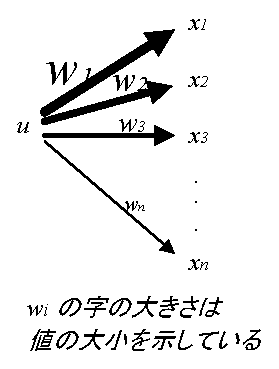
\epsfig{file=sfigure/c_gram.eps,scale=0.8}
  \caption{可制御グラミアン}
  \label{fig:c_gram}
 \end{center}
\end{minipage}
\begin{minipage}{5cm}
 \begin{center}
　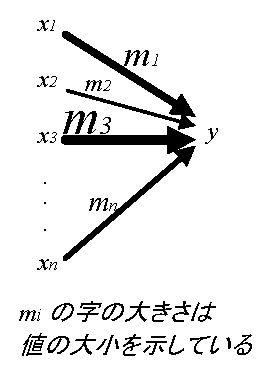
\epsfig{file=sfigure/o_gram.eps,scale=0.8}
  \caption{可観測グラミアン}
  \label{fig:o_gram}
 \end{center}
\end{minipage}
\end{center}
\end{figure}
\end{frame}

%%%%%%%%%%%%%%%%%%%%%%%%%%%%%%%%%%%%%%%%%%%%%%%%%%%%%%%%%%%%%%%
\begin{frame}[t]
\frametitle{2.8.1 可制御グラミアンの定義とその性質}
%-------------------------------------------------------------

グラミアンは数値計算でも重要な役割を果たしている．
\\[3mm]

例えば，$w_i$と$w_j$の大きさが極端に異なる場合には，シミュレーションで応答を計算した場合に$x_i$と$x_j$の大きさの違いが極端に異なることが予想される．この場合，数値計算上のケタ落ちなどの問題が発生する場合があるので注意する必要がある．
\\[3mm]

このようなときには後に述べる平衡実現のように状態の座標変換を用いてシミュレーションを行う必要がある．
\end{frame}

%%%%%%%%%%%%%%%%%%%%%%%%%%%%%%%%%%%%%%%%%%%%%%%%%%%%%%%%%%%%%%%
\begin{frame}[t]
\frametitle{2.8.2 可観測グラミアンの定義とその性質}
%-------------------------------------------------------------

\subsection{可観測グラミアンの定義とその性質}

\noindent
可観測グラミアンの定義
\begin{align}
	M = \int_{0}^{\infty} e^{A^T t} C^T C e^{At} dt
\end{align}
可観測グラミアンは次のリアプノフ方程式の正定解として求められる．
\begin{align}
	A^T M + M A = - C^T C
\end{align}
\end{frame}

%%%%%%%%%%%%%%%%%%%%%%%%%%%%%%%%%%%%%%%%%%%%%%%%%%%%%%%%%%%%%%%
\begin{frame}[t]
\frametitle{2.8.2 可観測グラミアンの定義とその性質}
%-------------------------------------------------------------
入力を$u(t)=0$, $t \in [0, \infty)$，初期状態を$x(0)=x_0$とするとき，（未来の）出力のエネルギーは可観測グラミアンを使って次のように表される．
\begin{align}
	\int_{0}^{\infty} y^T(t) y(t) \ dt = x_0^T M x_0
\end{align}
この式を理解するために$M$が$2 \times 2$で対角行列の場合を考える．
\begin{align}
	M = 
	\left(\begin{array}{cc}
         m_1 & 0 \\
	 0   & m_2 
	\end{array}\right)
\end{align}
この場合
\begin{align}
	\int_{0}^{\infty} y^T(t) y(t) \ dt 
	=
	\left(\begin{array}{cc}
         x_1(0) & x_2(0) 
	\end{array}\right)
	\left(\begin{array}{cc}
         m_1 & 0 \\
	 0   & m_2 
	\end{array}\right)
	\left(\begin{array}{c}
         x_1(0)\\
	 x_2(0) 
	\end{array}\right)
\end{align}
となる．
\end{frame}

%%%%%%%%%%%%%%%%%%%%%%%%%%%%%%%%%%%%%%%%%%%%%%%%%%%%%%%%%%%%%%%
\begin{frame}[t]
\frametitle{2.8.2 可観測グラミアンの定義とその性質}
%-------------------------------------------------------------
このとき，$\int_{0}^{\infty} y^T(t) y(t) \ dt =1$となる$x(0)$には
\begin{align}
	\left(\begin{array}{c}
         x_1(0)\\
	 x_2(0) 
	\end{array}\right)
	= 
	\left(\begin{array}{c}
         \sqrt{m_1^{-1}}\\
	 0 
	\end{array}\right)
	, \ \ \ \ 
	\left(\begin{array}{c}
         x_1(0)\\
	 x_2(0) 
	\end{array}\right)
	= 
	\left(\begin{array}{c}
         0\\
	 \sqrt{m_2^{-1}} 
	\end{array}\right)
\end{align}
等がある．
\\[3mm]

これは$m_i$が大きいほど，小さな$x_i(0)$で$\int_{0}^{\infty} y^T(t) y(t) \ dt =1$となることを意味し，状態$x_i$が出力に大きな影響を及ぼすことを意味している．
\\[3mm]

このように可観測グラミアンは状態の出力への影響の度合いを示している．
(Fig,\ref{fig:o_gram}は可観測グラミアンが$\mbox{diag}(m_1, m_2, \cdots, m_n)$の場合の状態が出力に及ぼす影響の大きさを表わしている．ここで図中の$m_i$の字の大きさは値の大きさを示している)


\end{frame}

%%%%%%%%%%%%%%%%%%%%%%%%%%%%%%%%%%%%%%%%%%%%%%%%%%%%%%%%%%%%%%%
\begin{frame}[t]
\frametitle{2.8.3 グラミアンに関する証明\\ (可制御グラミアンとリアプノフ方程式)}
%-------------------------------------------------------------
\subsection{グラミアンに関する証明}

\subsubsection{可制御グラミアンとリアプノフ方程式}

遷移行列の性質より$\frac{d}{dt} e^{At} = A e^{At} = e^{At} A$となることと，
$A$が安定であることより$e^{A \infty}=0$であることに注意して，次の積分
\begin{align}
	\int_{-\infty}^{0} \frac{d}{dt}e^{-At} B B^T e^{-A^T t} d t
\end{align}
を２つの方法で計算する．
\end{frame}

%%%%%%%%%%%%%%%%%%%%%%%%%%%%%%%%%%%%%%%%%%%%%%%%%%%%%%%%%%%%%%%
\begin{frame}[t]
\frametitle{2.8.3 グラミアンに関する証明\\ (可制御グラミアンとリアプノフ方程式)}
%-------------------------------------------------------------
\begin{align}
	\int_{-\infty}^{0} \frac{d}{dt}e^{-At} B B^T e^{-A^T t} d t
	&= \left[ e^{-At} B B^T e^{-A^T t} \right]_{-\infty}^0 = B B^T
\\
	\int_{-\infty}^{0} \frac{d}{dt}e^{-At} B B^T e^{-A^T t} d t
	&= \int_{-\infty}^{0}  -A e^{-At} B B^T e^{-A^T t} d t
\nonumber \\
	& \hspace*{1cm}
	   +\int_{-\infty}^{0} e^{-At} B B^T e^{-A^T t} \{-A^T\} d t
\nonumber \\
	&= -A W  - W A^T
\end{align}
よって
\begin{align}
	AW + W A^T = - B B^T
\end{align}

\end{frame}

%%%%%%%%%%%%%%%%%%%%%%%%%%%%%%%%%%%%%%%%%%%%%%%%%%%%%%%%%%%%%%%
\begin{frame}[t]
\frametitle{2.8.3 グラミアンに関する証明\\ (可観測グラミアンとリアプノフ方程式)}
%-------------------------------------------------------------
\subsubsection{可観測グラミアンとリアプノフ方程式}

前節と同様に証明できる．（演習）

\end{frame}

%%%%%%%%%%%%%%%%%%%%%%%%%%%%%%%%%%%%%%%%%%%%%%%%%%%%%%%%%%%%%%%
\begin{frame}[t]
\frametitle{2.8.3 グラミアンに関する証明\\ (可制御グラミアンと$x(0)$)}
%-------------------------------------------------------------
\subsubsection{可制御グラミアンと$x(0)$}

状態の入力応答は初期時刻を$t=0$とすると
\begin{align}
	x(t)= e^{At}x(0) + \int_{0}^{t} e^{A(t-\tau)}Bu(\tau) \ d \tau
\end{align}
と表される．初期時刻を$-\infty$とし，$x(0)$を求めれば
\begin{align}
	x(0) &= e^{A(0-(-\infty))}x(-\infty) + \int_{-\infty}^{0} e^{A(0-\tau)}Bu(\tau) \ d \tau
\nonumber \\
	&= e^{A(\infty)}x(-\infty) + \int_{-\infty}^{0} e^{-A\tau}Bu(\tau) \ d \tau
\end{align}
となる．
\end{frame}

%%%%%%%%%%%%%%%%%%%%%%%%%%%%%%%%%%%%%%%%%%%%%%%%%%%%%%%%%%%%%%%
\begin{frame}[t]
\frametitle{2.8.3 グラミアンに関する証明\\ (可制御グラミアンと$x(0)$)}
%-------------------------------------------------------------
ここで$A$は安定であること
より$e^{A\infty}=0$となるから
\begin{align}
	x(0) 
	&= \int_{-\infty}^{0} e^{-A\tau}Bu(\tau) \ d \tau
\end{align}
となる．ここで$u(t)=u_*(t) = B^T e^{-A^T t} W^{-1} x_0$を代入すれば
\begin{align}
	x(0) 
	&= \int_{-\infty}^{0} e^{-A\tau}B B^T e^{-A^T \tau} W^{-1} x_0 \ d \tau
\nonumber \\
	&= \int_{-\infty}^{0} e^{-A\tau}B B^T e^{-A^T \tau} \ d \tau \ W^{-1} x_0 \nonumber \\
	&= W W^{-1} x_0 = x_0
\end{align}
となる．

\end{frame}

%%%%%%%%%%%%%%%%%%%%%%%%%%%%%%%%%%%%%%%%%%%%%%%%%%%%%%%%%%%%%%%
\begin{frame}[t]
\frametitle{2.8.3 グラミアンに関する証明 ($u_*$の最小性)}
%-------------------------------------------------------------
\subsubsection{$u_*$の最小性}

前節の証明より$u(t)=u_*(t) = B^T e^{-A^T t} W^{-1} x_0$, $t\in(-\infty,0]$により状態は$t=0$で$x(0)=x_0$になることが証明された．これがエネルギー最小の入力であることは以下のように証明できる．
\\[3mm]

いま，次の入力
\begin{align}
	u(t)=u_*(t)+ \tilde{u}(t) = B^T e^{-A^T t} W^{-1} x_0 + \tilde{u}(t)
\end{align}
によっても状態が$x(0)=x_0$となると仮定する．
\end{frame}

%%%%%%%%%%%%%%%%%%%%%%%%%%%%%%%%%%%%%%%%%%%%%%%%%%%%%%%%%%%%%%%
\begin{frame}[t]
\frametitle{2.8.3 グラミアンに関する証明 ($u_*$の最小性)}
%-------------------------------------------------------------
このとき，
\begin{align}
	x(0) 
	&= \int_{-\infty}^{0} e^{-A\tau}B u(\tau) \ d \tau
\nonumber \\
	&= \int_{-\infty}^{0} e^{-A\tau}B \{u_*(\tau) + \tilde{u}(\tau) \} \ d \tau
\nonumber \\
	&= \int_{-\infty}^{0} e^{-A\tau}B u_*(\tau)  \ d \tau
	   + \int_{-\infty}^{0} e^{-A\tau}B \tilde{u}(\tau) \ d \tau
\nonumber \\
	&= x_0+ \int_{-\infty}^{0} e^{-A\tau}B \tilde{u}(\tau) \ d \tau
\end{align}
と$x(0)=x_0$より
\begin{align}
	\int_{-\infty}^{0} e^{-A\tau}B \tilde{u}(\tau) \ d \tau = 0
\end{align}
となる．
\end{frame}

%%%%%%%%%%%%%%%%%%%%%%%%%%%%%%%%%%%%%%%%%%%%%%%%%%%%%%%%%%%%%%%
\begin{frame}[t]
\frametitle{2.8.3 グラミアンに関する証明 ($u_*$の最小性)}
%-------------------------------------------------------------

\footnotesize
この$u(t)$のエネルギーを計算すれば
\begin{align}
	&\int_{-\infty}^{0} u^T(t) u(t) \ dt
\nonumber \\
	&= \int_{-\infty}^{0} 
		(B^T e^{-A^T t} W^{-1} x_0 + \tilde{u}(t))^T 
		(B^T e^{-A^T t} W^{-1} x_0 + \tilde{u}(t)) \ dt
\nonumber \\
	&= \int_{-\infty}^{0} 
		x_0^T W^{-1} e^{-A t} B B^T e^{-A^T t} W^{-1} x_0
		+ \tilde{u}^T(t) \tilde{u}(t) 
%\nonumber \\
%	& \hspace*{2cm}
		+ 2 x_0^T W^{-1} e^{-A t} B \tilde{u}(t) \ dt
\nonumber \\
	&= \int_{-\infty}^{0} 
		x_0^T W^{-1} e^{-A t} B B^T e^{-A^T t} W^{-1} x_0 \ dt
		+ \int_{-\infty}^{0} \tilde{u}^T(t) \tilde{u}(t) \ dt
%\nonumber \\ & \hspace{2cm}
		+ 2 x_0^T W^{-1} \int_{-\infty}^{0} e^{-A t} B \tilde{u}(t) \ dt
\nonumber \\
	&= \int_{-\infty}^{0} 
		x_0^T W^{-1} e^{-A t} B B^T e^{-A^T t} W^{-1} x_0 \ dt
		+ \int_{-\infty}^{0} \tilde{u}^T(t) \tilde{u}(t) \ dt
\nonumber \\
	&= x_0^T W^{-1} \left \{ \int_{-\infty}^{0} 
		 e^{-A t} B B^T e^{-A^T t} \ dt \right \} W^{-1} x_0 
		+ \int_{-\infty}^{0} \tilde{u}^T(t) \tilde{u}(t) \ dt
\nonumber \\
	&= x_0^T W^{-1} W W^{-1} x_0 
		+ \int_{-\infty}^{0} \tilde{u}^T(t) \tilde{u}(t) \ dt
\nonumber \\
	&= x_0^T W^{-1} x_0 
	   + \int_{-\infty}^{0} \tilde{u}^T(t) \tilde{u}(t) \ dt
\end{align}
これを最小とするのは$\tilde{u}=0$の場合であり，その最小値は$x_0^T W^{-1} x_0$となる．

\end{frame}

%%%%%%%%%%%%%%%%%%%%%%%%%%%%%%%%%%%%%%%%%%%%%%%%%%%%%%%%%%%%%%%
\begin{frame}[t]
\frametitle{2.8.4 平衡実現}
%-------------------------------------------------------------



\subsection{平衡実現}

可制御グラミアンは入力の状態への寄与率を，可観測グラミアンは状態の出力への寄与率を表している．これらを平衡させるつまり，可制御グラミアン$W$と可観測グラミアン$M$を一致させ，対角化するように状態の座標変換をすることがある．これを平衡実現と呼ぶ．
\\[3mm]

このようにするとひとつの状態$x_i$の入力からの寄与率と出力への寄与率が等しくなる．このような状態方程式は数値計算が安定になることがわかっており，計算機内でコントローラを実現する場合に用いられることが多い．

\end{frame}

%%%%%%%%%%%%%%%%%%%%%%%%%%%%%%%%%%%%%%%%%%%%%%%%%%%%%%%%%%%%%%%
\begin{frame}[t]
\frametitle{2.8.4 平衡実現}
%-------------------------------------------------------------

座標変換を
\begin{align}
	x=T\bar{x}
\end{align}で定義する．このとき座標変換後の可制御グラミアン$\bar{W}$は
\begin{align}
	\bar{W}= T^{-1} W T^{-T}
\end{align}
と，座標変換後の可観測グラミアン$\bar{M}$は
\begin{align}
	\bar{M}= T^T M T
\end{align}
と表される（演習）．
\end{frame}

%%%%%%%%%%%%%%%%%%%%%%%%%%%%%%%%%%%%%%%%%%%%%%%%%%%%%%%%%%%%%%%
\begin{frame}[t]
\frametitle{2.8.4 平衡実現}
%-------------------------------------------------------------
ここで
\begin{align}
	\bar{W}=\bar{M}= \Sigma 
	= 
	\left(\begin{array}{cccc}
         \sigma_1 &          &       &  \\
                  & \sigma_2 &       &  \\
                  &          & \ddots &  \\
                  &          &       &  \sigma_n
	\end{array}\right)
\end{align}
となる$T$を求める．明らかに
\begin{align}
	\bar{W} \bar{M} &= \Sigma^2
\\
	\bar{W} \bar{M} &= T^{-1} W T^{-T} T^T M T = T^{-1} W M T
\end{align}
となるから
\begin{align}
	T^{-1} W M T &= \Sigma^2
\end{align}
となる．
\end{frame}

%%%%%%%%%%%%%%%%%%%%%%%%%%%%%%%%%%%%%%%%%%%%%%%%%%%%%%%%%%%%%%%
\begin{frame}[t]
\frametitle{2.8.4 平衡実現}
%-------------------------------------------------------------
$M$は正定行列であることから正則行列$H$を用いて$M=H^T H$と分解できる．これを代入すると
\begin{align}
	T^{-1} W H^T H T &= \Sigma^2
\end{align}
これを次のように変形する
\begin{align}
	\Sigma^2 &= T^{-1} W H^T H T 
		= T^{-1} H^{-1} H W H^T H T 
		= (HT)^{-1} HWH^T (HT)
\end{align}
これは$HWH^T$が$\Sigma^2$と対角化できることを示している．
\end{frame}

%%%%%%%%%%%%%%%%%%%%%%%%%%%%%%%%%%%%%%%%%%%%%%%%%%%%%%%%%%%%%%%
\begin{frame}[t]
\frametitle{2.8.4 平衡実現}
%-------------------------------------------------------------
一方$HWH^T$は対称行列であるから直交行列$U$($U^TU=I)$を用いて対角がすることもできるはずである．このときも$\Sigma^2$に対角化できるはずであるから
\begin{align}
	U^T HWH^T U & = \Sigma^2
\end{align}
なる$U$が存在する．
\end{frame}

%%%%%%%%%%%%%%%%%%%%%%%%%%%%%%%%%%%%%%%%%%%%%%%%%%%%%%%%%%%%%%%
\begin{frame}[t]
\frametitle{2.8.4 平衡実現}
%-------------------------------------------------------------
これらを用いて$T$を
\begin{align}
	T=H^{-1} U \Sigma^{1/2}
	, \ \ \ \
	T^{-1} = \Sigma^{-1/2} U^T H
\end{align}
と定義すると
\begin{align}
	\bar{W}= T^{-1} W T^{-T} 
	& =  \Sigma^{-1/2} U^T H W H^T U \Sigma^{-1/2} 
\nonumber \\
	& =  \Sigma^{-1/2} \Sigma^2 \Sigma^{-1/2} = \Sigma
\end{align}
と，座標変換後の可観測グラミアン$\bar{M}$は
\begin{align}
	\bar{M}= T^T M T 
	& = \Sigma^{1/2} U^T H^{-T}M H^{-1} U \Sigma^{1/2}
\nonumber \\
	& = \Sigma^{1/2} U^T H^{-T} H^T H H^{-1} U \Sigma^{1/2} = \Sigma
\end{align}
となり，平衡実現が完成する．
\end{frame}

%%%%%%%%%%%%%%%%%%%%%%%%%%%%%%%%%%%%%%%%%%%%%%%%%%%%%%%%%%%%%%%
\begin{frame}[t]
\frametitle{2.8.4 平衡実現}
%-------------------------------------------------------------

グラミアンの値$\sigma_i$が小さい状態は入力の寄与率も出力への寄与率も小さいので無視できることがある．このように状態方程式の次元を下げる方法をbalanced trancationと呼ぶことがある．


\begin{figure}[htbp]
 \begin{center}
　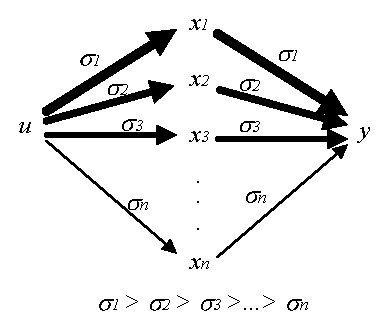
\epsfig{file=sfigure/b_gram.eps,scale=1}
  \caption{平衡実現}
  \label{fig:b_gram}
 \end{center}
\end{figure}


\pagebreak


\end{frame}

%%%%%%%%%%%%%%%%%%%%%%%%%%%%%%%%%%%%%%%%%%%%%%%%%%%%%%%%%%%%%%%
\begin{frame}[t]
\frametitle{2.9 安定性の定義}
%-------------------------------------------------------------
\section{安定性の定義}

状態方程式$\dot{x}=f(x), \ f(0)=0$に対してその{\bf 平衡状態(equilibrium state)}$x=0$を考える．任意の$\epsilon>0$に対してある$\delta$が存在して$\vert x(0) \vert < \delta \ \Rightarrow \ \vert x(t) \vert < \epsilon$が成り立つとき$x=0$は{\bf 安定(stable)}であるという．安定でないとき{\bf 不安定(unstable)}という．また，安定で，$\vert x(0) \vert < \delta \ \Rightarrow \ \lim_{t \rightarrow \infty} x(t) =0$のとき，{\bf 漸近安定(asymptotically stable)}という．また，ある定数$M>0$と$\alpha>0$が存在し，$\vert x(t) \vert < M e^{-\alpha t} x(0)$となるとき{\bf 指数安定(exponentially stable)}という．

\begin{figure}[htbp]
 \begin{center}
　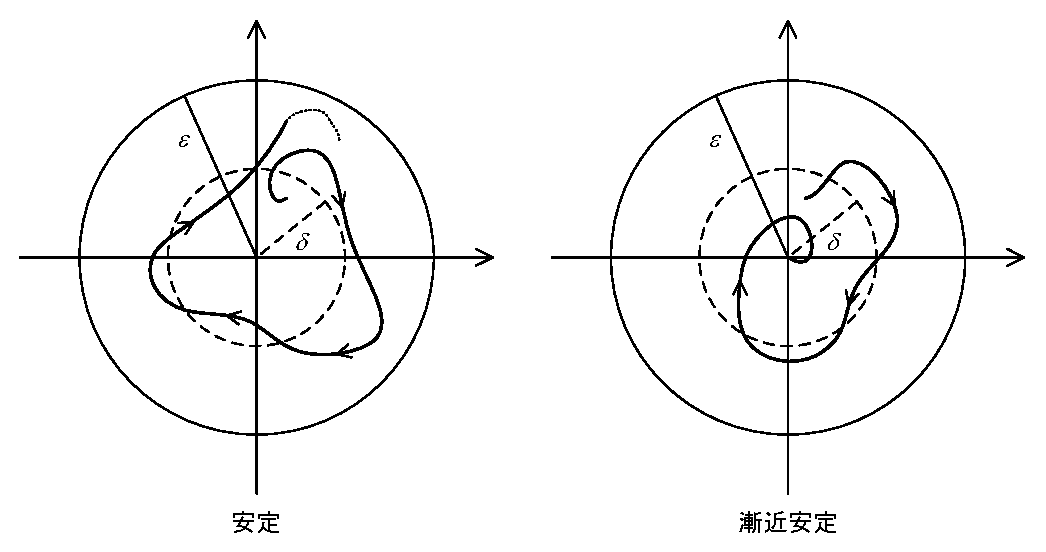
\epsfig{file=sfigure/stability.eps,scale=0.5}
  \caption{安定と漸近安定}
  \label{fig:stability}
 \end{center}
\end{figure}
\end{frame}


